\documentclass[../main.tex]{subfiles}
\begin{document}

\ifSubfilesClassLoaded{\mainmatter}{}

\chapter{Introduction}
\label{ch:intro}
The first direct evidence for point-like constituents in the nucleon came
from the deep-inelastic scattering (DIS) experiments at SLAC~\cite{breidenbach1969},
which led to the introduction of quantum chromodynamics (QCD)~\cite{fritzsch1972,fritzsch1973}.
According to QCD, nucleons are composed of quarks and gluons (collectively known as partons),
bound together through the exchange of gluons. One key feature of QCD is the ``asymptotic freedom'':
the effective coupling of QCD goes to zero at zero distance~\cite{gross1973,politzer1973}.
This allows short-distance processes to be analyzed using perturbative methods.
However, the effective coupling becomes progressively larger at longer distance,
ultimately being strong enough to lead to the confinement of quarks and gluons.
In the long distance regime perturbation theory clearly fails.
An alternative approach is used in the regime, known as lattice QCD~\cite{wilson1974},
which involves replacing the space-time continuum by discrete lattice of points.
Although enormous progress have been made in lattice QCD calculations, they are limited
both in achievable accuracy and in the observables that can be predicted.
Much of the predictive power of QCD is contained in factorization theorems~\cite{collins1989}.
QCD factorization separate hadronic collisions into long- and short-distance effects.
While perturbative expansion of QCD has successfully described the short-distance hard scattering,
the long-distance effects, such as the internal structure of hadrons,
could not be calculated with perturbative QCD, and have to be determined experimentally or via lattice QCD.

This thesis presents results from SeaQuest, a fixed-target experiment at Fermilab.
The primary goal of SeaQuest is to investigate the antiquark structures
in the proton from the detection of high mass $\mu^+\mu^-$ pairs produced in
the interaction of a \SI{120}{\GeV} proton beam with various targets, including liquid \ce{^1H} and \ce{^2H}.
The $\mu^+\mu^-$ data consist of multiple components, notably the Drell-Yan continuum,
and the  $J/\psi$ and $\psi^\prime$ resonances.
Both the Drell-Yan and the $J/\psi$ ($\psi^\prime$) data can be used to probe
the antiquark structures in the proton.
The $J/\psi$ ($\psi^\prime$) production is further sensitive to the gluon structure in the proton.

This thesis is organized as follows. After reviewing the early studies
on the nucleon structure and the DIS in this chapter,
the Drell-Yan process and the kinematic variables are summarized in
\cref{ch:DY}. The charmonium production and gluon distribution are discussed
in \cref{ch:jpsi}. The SeaQuest experiment is described in \cref{M-ch:seaquest}.
\Cref{M-ch:analysis} covers the procedure for data analysis. The measured $J/\psi$ ($\psi'$)
cross sections and the $\sigma_{pd}/2\sigma_{pp}$ cross section ratio for both $J/\psi$ and Drell-Yan process
are presented in \cref{M-ch:result}, followed by a summary and a discussion of future prospects
in \cref{M-ch:conclusion}.

\section{Early Evidence of the Internal Structure of Nucleon}
The first evidence of nucleons being composite particles came from the
measurements of their magnetic moments. For spin $1/2$ elementary particles, the
magnetic moment can be expressed as
\begin{equation}
	\mu = \frac{g}{2} \frac{e\hbar}{2m},
\end{equation}
with $g$ expected to be \num{2}. Such measurement was first carried out in 1933.
And the $g$ factor for proton is found to be significantly greater than \num{2}~\cite{frisch1933}.
Since neutron is a neutral particle, it was expected
to have a zero magnetic moment. The neutron magnetic moment was later measured
to be non-zero, suggesting that proton and neutron are
both composite particles~\cite{rabi1934}. The current values of the $g$ factors
for the charged leptons and nucleons are listed in \cref{tab:g-factor}.
The deviation from \num{2} for electrons and muons are expected from higher-order corrections,
and have been studied extensively~\cite{fan2023,abi2021}.
{
\sisetup{separate-uncertainty = false}
\begin{table}[h!]
	\centering
	\caption{$g$ factor for $e$, $\mu$, $p$ and $n$ \cite{workman2022}.}
	\label{tab:g-factor}
	\begin{tabular}{|c|c|c|c|c|}
		\hline
		    & $e$                        & $\mu$                  & $p$                    & $n$                   \\ \hline
		$g$ & \num{2.00231930436256(35)} & \num{2.0023318418(13)} & \num{5.5856946893(16)} & \num{-3.82608545(90)} \\ \hline
	\end{tabular}
\end{table}
}

The first insight into the internal structure of the nucleon came from the
electron proton elastic scattering experiments~\cite{hofstadter1956} in the
1950s. The electron-proton elastic scattering cross section at angle $\theta$ in the laboratory
frame can be expressed in the Rosenbluth formula~\cite{rosenbluth1950}
\begin{equation}
	\dv{\sigma}{\Omega} = \frac{\alpha^2}{4E^2 \sin^2\left(\theta/2\right)}
	\frac{E^\prime}{E} \left( \frac{G_E^2+\tau G_M^2}{1+\tau} \cos^2
	\frac{\theta}{2} + 2\tau G_M^2 \sin^2 \frac{\theta}{2}\right)
	\label{eq:ep_cs},
\end{equation}
where $\tau = \frac{Q^2}{4m_p^2}$.
And $E$, $E^\prime$ are the initial and final energy of the scattered electron.
The electric ($G_E\left(Q^2\right)$) and magnetic ($G_M\left(Q^2\right)$) form
factors are functions of the negative squared of four momentum $Q^2$ of the virtual photon. At
low-$Q^2$ limit, these form factors can be interpreted as the Fourier transforms
of the charge and magnetic moment distribution of the nucleon, and the mean squared
charge radius can be obtained from the first derivative of the electric form factor.
\begin{equation}
	\expval{r^2_E}=-6\eval{\dv{G_E\left(Q^2\right)}{Q^2}}_{Q^2=0}.
\end{equation}
This interpretation is however later questioned in Refs.~\cite{miller2007,miller2019}.
The author argued that a three-dimensional charge density, in the strict sense of a
probability interpretation, cannot be defined for a nucleon (as a relativistic system of quarks and gluons)
because the initial and final state proton wave functions are different. Instead,
a two-dimensional charge density can be defined in the infinite momentum frame as
\begin{equation}
	\rho(b)=\int^\infty_0 \frac{\dd{Q}Q}{2\pi} J_0(Qb)\frac{G_E^2(Q^2)+\tau G_M^2(Q^2)}{1+\tau},
\end{equation}
where $b$ is the impact parameter and $J_0$ is a cylindrical Bessel function.
\Cref{fig:charge}
shows a recent extraction of the proton and neutron transverse charge density from the
form factors, taken from Ref.~\cite{miller2007}. In particular, it was found that
the neutron has a negatively charged center and surrounded by a positive cloud.
\begin{figure}[hbp!]
	\centering
	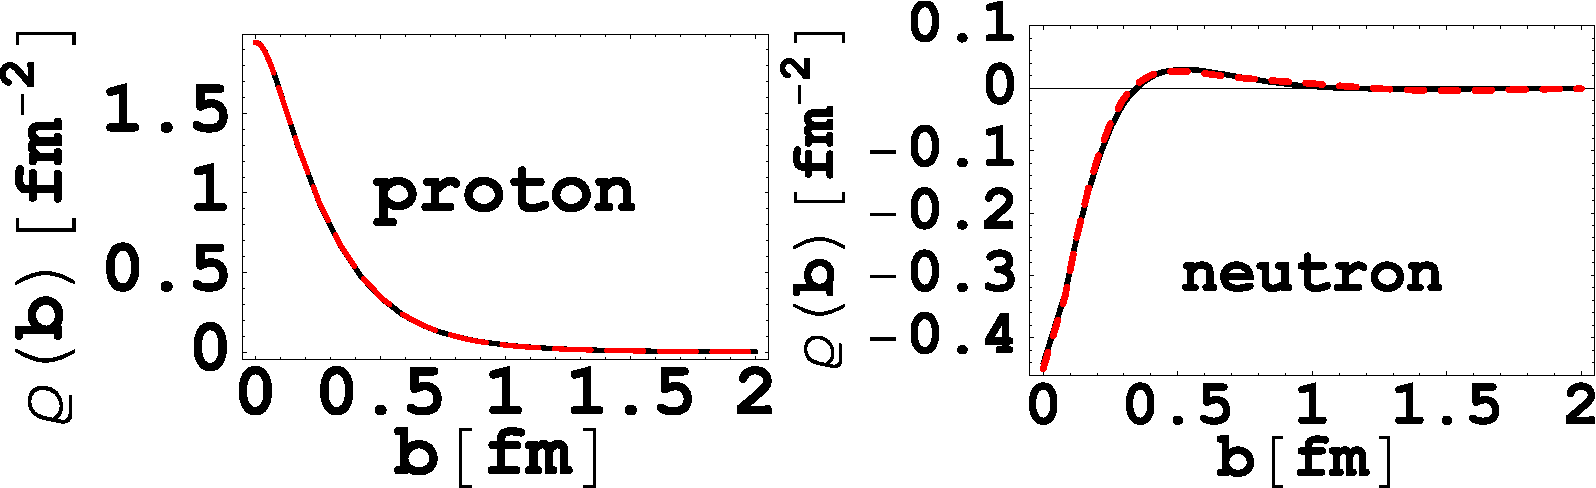
\includegraphics[width=0.9\linewidth]{charge_distribution_rotated}
	\caption{The proton charge density (left panel) and neutron charge density
		(right panel), taken from Ref.~\cite{miller2007}.}
	\label{fig:charge}
\end{figure}
These results further illustrate the internal structure of the nucleon.

In the 1960s, the quark model was proposed independently by Gell-Mann~\cite{gell-mann1964} and Zweig ~\cite{zweig1964a, zweig1964}
to understand the growing number of new particles discovered throughout the 1940s and 1950s.
In the quark model, the baryons are made up of three quarks and the mesons are made up
of a quark and an antiquark. They can be organized as shown in \cref{fig:Octet}.
The magnetic moment of the proton can then be expressed as the sum of the magnetic moment
from the individual quarks. The proton consists of $uud$ and the neutron consists of $udd$,
requiring the wavefunction to be symmetric in both flavor and spin, and the flavor-spin wavefunction of a proton with
spin up is given by
\begin{equation}
	\begin{split}
		\ket{p,\uparrow}= & \Bigl\{\frac{1}{2}\ket{\uparrow\downarrow\uparrow-\downarrow\uparrow\uparrow}\ket{udu-duu} + \frac{1}{2}\ket{\uparrow\uparrow\downarrow-\uparrow\downarrow\uparrow}\ket{uud-udu} \\
		                  & +\frac{1}{2}\ket{\uparrow\uparrow\downarrow-\downarrow\uparrow\uparrow}\ket{uud-duu}\Bigr\} \frac{\sqrt{2}}{3}.
	\end{split}
\end{equation}
And the magnetic moments are now given by
\begin{align}
	\mu_p & = \frac{4}{3}\mu_u-\frac{1}{3}\mu_d,  \\
	\mu_n & = -\frac{1}{3}\mu_u+\frac{4}{3}\mu_d.
\end{align}
If we also assumed that $u$ and $d$ quarks share the same mass, the quark model
then predicts the ratio $\mu_p/\mu_n=-2/3$ which is impressively close to the measured ratio of
\num{0.6849793(3)}~\cite{workman2022}.
\begin{figure}[h!]
	\centering
	\begin{subfigure}{0.45\linewidth}
		

\tikzset{every picture/.style={line width=0.75pt}} %set default line width to 0.75pt        

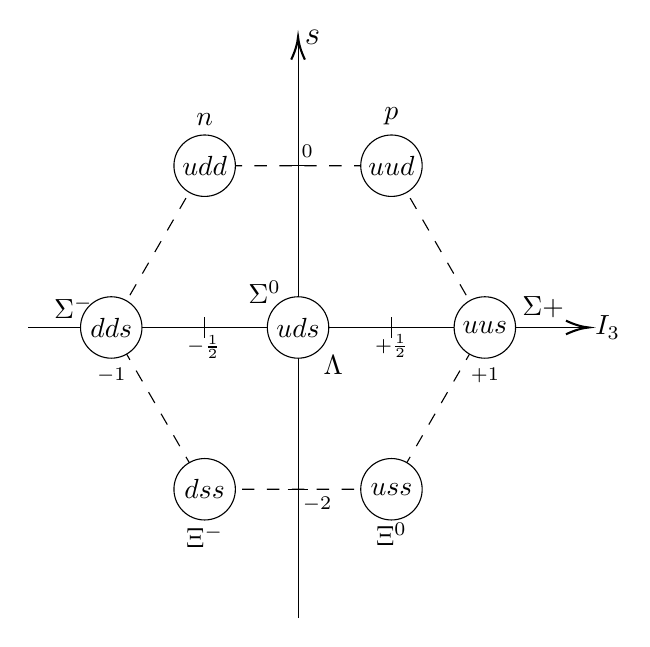
\begin{tikzpicture}[x=0.75pt,y=0.75pt,yscale=-1,xscale=1]
%uncomment if require: \path (0,585); %set diagram left start at 0, and has height of 585

%Shape: Regular Polygon [id:dp3461512214390913] 
\draw  [dash pattern={on 4.5pt off 4.5pt}] (360,280) -- (315,357.94) -- (225,357.94) -- (180,280) -- (225,202.06) -- (315,202.06) -- cycle ;
%Straight Lines [id:da7975119261953387] 
\draw    (140,280) -- (408,280) ;
\draw [shift={(410,280)}, rotate = 180] [color={rgb, 255:red, 0; green, 0; blue, 0 }  ][line width=0.75]    (10.93,-3.29) .. controls (6.95,-1.4) and (3.31,-0.3) .. (0,0) .. controls (3.31,0.3) and (6.95,1.4) .. (10.93,3.29)   ;
%Straight Lines [id:da49187250319695275] 
\draw    (270,420) -- (270,142) ;
\draw [shift={(270,140)}, rotate = 90] [color={rgb, 255:red, 0; green, 0; blue, 0 }  ][line width=0.75]    (10.93,-3.29) .. controls (6.95,-1.4) and (3.31,-0.3) .. (0,0) .. controls (3.31,0.3) and (6.95,1.4) .. (10.93,3.29)   ;
%Straight Lines [id:da04662903115423256] 
\draw    (225,275) -- (225,285) ;
%Straight Lines [id:da6078809997154113] 
\draw    (315,275) -- (315,285) ;
%Shape: Circle [id:dp2506066338504991] 
\draw  [fill={rgb, 255:red, 255; green, 255; blue, 255 }  ,fill opacity=1 ] (210.2,202.06) .. controls (210.2,193.88) and (216.83,187.26) .. (225,187.26) .. controls (233.17,187.26) and (239.8,193.88) .. (239.8,202.06) .. controls (239.8,210.23) and (233.17,216.86) .. (225,216.86) .. controls (216.83,216.86) and (210.2,210.23) .. (210.2,202.06) -- cycle ;
%Shape: Circle [id:dp49323091495562255] 
\draw  [fill={rgb, 255:red, 255; green, 255; blue, 255 }  ,fill opacity=1 ] (300.2,202.06) .. controls (300.2,193.88) and (306.83,187.26) .. (315,187.26) .. controls (323.17,187.26) and (329.8,193.88) .. (329.8,202.06) .. controls (329.8,210.23) and (323.17,216.86) .. (315,216.86) .. controls (306.83,216.86) and (300.2,210.23) .. (300.2,202.06) -- cycle ;
%Shape: Circle [id:dp2780130541001513] 
\draw  [fill={rgb, 255:red, 255; green, 255; blue, 255 }  ,fill opacity=1 ] (165.2,280) .. controls (165.2,271.83) and (171.83,265.2) .. (180,265.2) .. controls (188.17,265.2) and (194.8,271.83) .. (194.8,280) .. controls (194.8,288.17) and (188.17,294.8) .. (180,294.8) .. controls (171.83,294.8) and (165.2,288.17) .. (165.2,280) -- cycle ;
%Shape: Circle [id:dp22149042815123876] 
\draw  [fill={rgb, 255:red, 255; green, 255; blue, 255 }  ,fill opacity=1 ] (345.2,280) .. controls (345.2,271.83) and (351.83,265.2) .. (360,265.2) .. controls (368.17,265.2) and (374.8,271.83) .. (374.8,280) .. controls (374.8,288.17) and (368.17,294.8) .. (360,294.8) .. controls (351.83,294.8) and (345.2,288.17) .. (345.2,280) -- cycle ;
%Shape: Circle [id:dp2315285626329665] 
\draw  [fill={rgb, 255:red, 255; green, 255; blue, 255 }  ,fill opacity=1 ] (210.2,357.94) .. controls (210.2,349.77) and (216.83,343.14) .. (225,343.14) .. controls (233.17,343.14) and (239.8,349.77) .. (239.8,357.94) .. controls (239.8,366.12) and (233.17,372.74) .. (225,372.74) .. controls (216.83,372.74) and (210.2,366.12) .. (210.2,357.94) -- cycle ;
%Shape: Circle [id:dp3088315424845015] 
\draw  [fill={rgb, 255:red, 255; green, 255; blue, 255 }  ,fill opacity=1 ] (300.2,357.94) .. controls (300.2,349.77) and (306.83,343.14) .. (315,343.14) .. controls (323.17,343.14) and (329.8,349.77) .. (329.8,357.94) .. controls (329.8,366.12) and (323.17,372.74) .. (315,372.74) .. controls (306.83,372.74) and (300.2,366.12) .. (300.2,357.94) -- cycle ;
%Shape: Circle [id:dp27152267435822064] 
\draw  [fill={rgb, 255:red, 255; green, 255; blue, 255 }  ,fill opacity=1 ] (255.2,280) .. controls (255.2,271.83) and (261.83,265.2) .. (270,265.2) .. controls (278.17,265.2) and (284.8,271.83) .. (284.8,280) .. controls (284.8,288.17) and (278.17,294.8) .. (270,294.8) .. controls (261.83,294.8) and (255.2,288.17) .. (255.2,280) -- cycle ;
%Straight Lines [id:da5232366045305828] 
\draw    (265,202.1) -- (275,202.1) ;
%Straight Lines [id:da5088485977717139] 
\draw    (265,357.94) -- (275,357.94) ;

% Text Node
\draw (272,140) node [anchor=west] [inner sep=0.75pt]  [font=\large]  {$s$};
% Text Node
\draw (412,280) node [anchor=west] [inner sep=0.75pt]    {$I_{3}$};
% Text Node
\draw (270.5,190.65) node [anchor=north west][inner sep=0.75pt]  [font=\fontsize{0.71em}{0.85em}\selectfont]  {$0$};
% Text Node
\draw (271.08,360.57) node [anchor=north west][inner sep=0.75pt]  [font=\fontsize{0.71em}{0.85em}\selectfont]  {$-2$};
% Text Node
\draw (180,298.2) node [anchor=north] [inner sep=0.75pt]  [font=\fontsize{0.71em}{0.85em}\selectfont]  {$-1$};
% Text Node
\draw (360,298.2) node [anchor=north] [inner sep=0.75pt]  [font=\fontsize{0.71em}{0.85em}\selectfont]  {$+1$};
% Text Node
\draw (315.09,282.28) node [anchor=north] [inner sep=0.75pt]  [font=\fontsize{0.71em}{0.85em}\selectfont]  {$+\frac{1}{2}$};
% Text Node
\draw (224.65,282.6) node [anchor=north] [inner sep=0.75pt]  [font=\fontsize{0.71em}{0.85em}\selectfont]  {$-\frac{1}{2}$};
% Text Node
\draw (225,202.06) node    {$udd$};
% Text Node
\draw (315,202.06) node    {$uud$};
% Text Node
\draw (180,280) node    {$dds$};
% Text Node
\draw (270,280) node    {$uds$};
% Text Node
\draw (360,280) node    {$uus$};
% Text Node
\draw (225,357.94) node    {$dss$};
% Text Node
\draw (315,357.94) node    {$uss$};
% Text Node
\draw (225,183.86) node [anchor=south] [inner sep=0.75pt]    {$n$};
% Text Node
\draw (315,183.86) node [anchor=south] [inner sep=0.75pt]    {$p$};
% Text Node
\draw (225,374.14) node [anchor=north] [inner sep=0.75pt]    {$\Xi ^{-}$};
% Text Node
\draw (315,373.14) node [anchor=north] [inner sep=0.75pt]    {$\Xi ^{0}$};
% Text Node
\draw (172.38,276.82) node [anchor=south east] [inner sep=0.75pt]    {$\Sigma ^{-}$};
% Text Node
\draw (376.8,276.6) node [anchor=south west] [inner sep=0.75pt]    {$\Sigma +$};
% Text Node
\draw (263,269.6) node [anchor=south east] [inner sep=0.75pt]    {$\Sigma ^{0}$};
% Text Node
\draw (281,292.4) node [anchor=north west][inner sep=0.75pt]    {$\Lambda $};


\end{tikzpicture}


		\caption{The baryon spin 1/2 octet.}
	\end{subfigure}
	\hspace{3mm}%
	\begin{subfigure}{0.45\linewidth}
		

\tikzset{every picture/.style={line width=0.75pt}} %set default line width to 0.75pt        

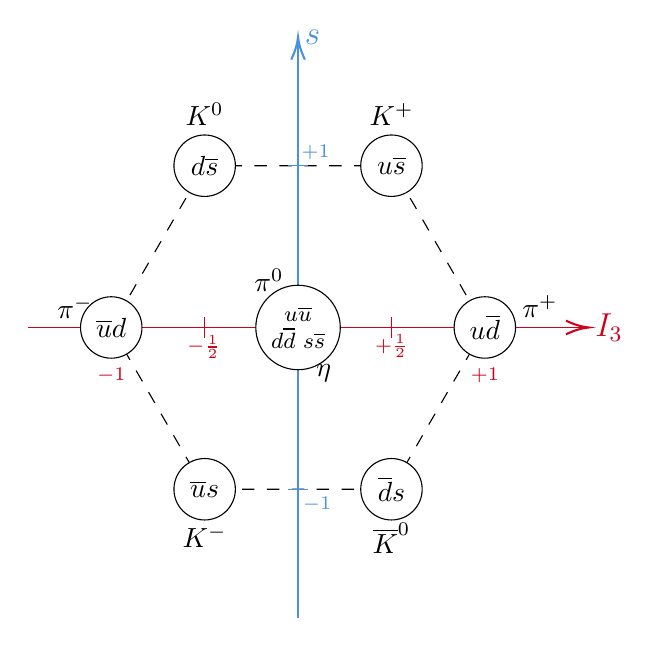
\begin{tikzpicture}[x=0.75pt,y=0.75pt,yscale=-1,xscale=1]
%uncomment if require: \path (0,312); %set diagram left start at 0, and has height of 312

%Shape: Regular Polygon [id:dp00036259320032794307] 
\draw  [dash pattern={on 4.5pt off 4.5pt}] (230,162) -- (185,239.94) -- (95,239.94) -- (50,162) -- (95,84.06) -- (185,84.06) -- cycle ;
%Straight Lines [id:da7432714490785992] 
\draw [color={rgb, 255:red, 208; green, 2; blue, 27 }  ,draw opacity=1 ]   (10,162) -- (278,162) ;
\draw [shift={(280,162)}, rotate = 180] [color={rgb, 255:red, 208; green, 2; blue, 27 }  ,draw opacity=1 ][line width=0.75]    (10.93,-3.29) .. controls (6.95,-1.4) and (3.31,-0.3) .. (0,0) .. controls (3.31,0.3) and (6.95,1.4) .. (10.93,3.29)   ;
%Straight Lines [id:da5800138783290809] 
\draw [color={rgb, 255:red, 74; green, 144; blue, 226 }  ,draw opacity=1 ]   (140,302) -- (140,24) ;
\draw [shift={(140,22)}, rotate = 90] [color={rgb, 255:red, 74; green, 144; blue, 226 }  ,draw opacity=1 ][line width=0.75]    (10.93,-3.29) .. controls (6.95,-1.4) and (3.31,-0.3) .. (0,0) .. controls (3.31,0.3) and (6.95,1.4) .. (10.93,3.29)   ;
%Straight Lines [id:da0424063895802933] 
\draw [color={rgb, 255:red, 208; green, 2; blue, 27 }  ,draw opacity=1 ]   (95,157) -- (95,167) ;
%Straight Lines [id:da5315540321645463] 
\draw [color={rgb, 255:red, 208; green, 2; blue, 27 }  ,draw opacity=1 ]   (185,157) -- (185,167) ;
%Shape: Circle [id:dp9016274878129079] 
\draw  [fill={rgb, 255:red, 255; green, 255; blue, 255 }  ,fill opacity=1 ] (80.2,84.06) .. controls (80.2,75.88) and (86.83,69.26) .. (95,69.26) .. controls (103.17,69.26) and (109.8,75.88) .. (109.8,84.06) .. controls (109.8,92.23) and (103.17,98.86) .. (95,98.86) .. controls (86.83,98.86) and (80.2,92.23) .. (80.2,84.06) -- cycle ;
%Shape: Circle [id:dp26967635701794923] 
\draw  [fill={rgb, 255:red, 255; green, 255; blue, 255 }  ,fill opacity=1 ] (170.2,84.06) .. controls (170.2,75.88) and (176.83,69.26) .. (185,69.26) .. controls (193.17,69.26) and (199.8,75.88) .. (199.8,84.06) .. controls (199.8,92.23) and (193.17,98.86) .. (185,98.86) .. controls (176.83,98.86) and (170.2,92.23) .. (170.2,84.06) -- cycle ;
%Shape: Circle [id:dp829825410707284] 
\draw  [fill={rgb, 255:red, 255; green, 255; blue, 255 }  ,fill opacity=1 ] (35.2,162) .. controls (35.2,153.83) and (41.83,147.2) .. (50,147.2) .. controls (58.17,147.2) and (64.8,153.83) .. (64.8,162) .. controls (64.8,170.17) and (58.17,176.8) .. (50,176.8) .. controls (41.83,176.8) and (35.2,170.17) .. (35.2,162) -- cycle ;
%Shape: Circle [id:dp7821465181120492] 
\draw  [fill={rgb, 255:red, 255; green, 255; blue, 255 }  ,fill opacity=1 ] (215.2,162) .. controls (215.2,153.83) and (221.83,147.2) .. (230,147.2) .. controls (238.17,147.2) and (244.8,153.83) .. (244.8,162) .. controls (244.8,170.17) and (238.17,176.8) .. (230,176.8) .. controls (221.83,176.8) and (215.2,170.17) .. (215.2,162) -- cycle ;
%Shape: Circle [id:dp050740490078981626] 
\draw  [fill={rgb, 255:red, 255; green, 255; blue, 255 }  ,fill opacity=1 ] (80.2,239.94) .. controls (80.2,231.77) and (86.83,225.14) .. (95,225.14) .. controls (103.17,225.14) and (109.8,231.77) .. (109.8,239.94) .. controls (109.8,248.12) and (103.17,254.74) .. (95,254.74) .. controls (86.83,254.74) and (80.2,248.12) .. (80.2,239.94) -- cycle ;
%Shape: Circle [id:dp8501124972426272] 
\draw  [fill={rgb, 255:red, 255; green, 255; blue, 255 }  ,fill opacity=1 ] (170.2,239.94) .. controls (170.2,231.77) and (176.83,225.14) .. (185,225.14) .. controls (193.17,225.14) and (199.8,231.77) .. (199.8,239.94) .. controls (199.8,248.12) and (193.17,254.74) .. (185,254.74) .. controls (176.83,254.74) and (170.2,248.12) .. (170.2,239.94) -- cycle ;
%Shape: Circle [id:dp12490437005601918] 
\draw  [fill={rgb, 255:red, 255; green, 255; blue, 255 }  ,fill opacity=1 ] (119.65,162) .. controls (119.65,150.76) and (128.76,141.65) .. (140,141.65) .. controls (151.24,141.65) and (160.35,150.76) .. (160.35,162) .. controls (160.35,173.24) and (151.24,182.35) .. (140,182.35) .. controls (128.76,182.35) and (119.65,173.24) .. (119.65,162) -- cycle ;
%Straight Lines [id:da10691295631235598] 
\draw [color={rgb, 255:red, 74; green, 144; blue, 226 }  ,draw opacity=1 ]   (135,84.06) -- (145,84.06) ;
%Straight Lines [id:da40035051048673465] 
\draw [color={rgb, 255:red, 74; green, 144; blue, 226 }  ,draw opacity=1 ]   (135,239.9) -- (145,239.9) ;

% Text Node
\draw (142,22) node [anchor=west] [inner sep=0.75pt]  [font=\large,color={rgb, 255:red, 74; green, 144; blue, 226 }  ,opacity=1 ]  {$s$};
% Text Node
\draw (282,162) node [anchor=west] [inner sep=0.75pt]  [font=\large,color={rgb, 255:red, 208; green, 2; blue, 27 }  ,opacity=1 ]  {$I_{3}$};
% Text Node
\draw (140.5,72.65) node [anchor=north west][inner sep=0.75pt]  [font=\fontsize{0.71em}{0.85em}\selectfont,color={rgb, 255:red, 74; green, 144; blue, 226 }  ,opacity=1 ]  {$+1$};
% Text Node
\draw (141.08,242.57) node [anchor=north west][inner sep=0.75pt]  [font=\fontsize{0.71em}{0.85em}\selectfont,color={rgb, 255:red, 74; green, 144; blue, 226 }  ,opacity=1 ]  {$-1$};
% Text Node
\draw (50,180.2) node [anchor=north] [inner sep=0.75pt]  [font=\fontsize{0.71em}{0.85em}\selectfont,color={rgb, 255:red, 208; green, 2; blue, 27 }  ,opacity=1 ]  {$-1$};
% Text Node
\draw (230,180.2) node [anchor=north] [inner sep=0.75pt]  [font=\fontsize{0.71em}{0.85em}\selectfont,color={rgb, 255:red, 208; green, 2; blue, 27 }  ,opacity=1 ]  {$+1$};
% Text Node
\draw (185.09,164.28) node [anchor=north] [inner sep=0.75pt]  [font=\fontsize{0.71em}{0.85em}\selectfont,color={rgb, 255:red, 208; green, 2; blue, 27 }  ,opacity=1 ]  {$+\frac{1}{2}$};
% Text Node
\draw (94.65,164.6) node [anchor=north] [inner sep=0.75pt]  [font=\fontsize{0.71em}{0.85em}\selectfont,color={rgb, 255:red, 208; green, 2; blue, 27 }  ,opacity=1 ]  {$-\frac{1}{2}$};
% Text Node
\draw (95,84.06) node    {$d\overline{s}$};
% Text Node
\draw (185,84.06) node    {$u\overline{s}$};
% Text Node
\draw (50,162) node    {$\overline{u} d$};
% Text Node
\draw (230,162) node    {$u\overline{d}$};
% Text Node
\draw (95,239.94) node    {$\overline{u} s$};
% Text Node
\draw (185,239.94) node    {$\overline{d} s$};
% Text Node
\draw (95,65.86) node [anchor=south] [inner sep=0.75pt]    {$K^{0}$};
% Text Node
\draw (185,65.86) node [anchor=south] [inner sep=0.75pt]    {$K^{+}$};
% Text Node
\draw (95,256.14) node [anchor=north] [inner sep=0.75pt]    {$K^{-}$};
% Text Node
\draw (185,255.14) node [anchor=north] [inner sep=0.75pt]    {$\overline{K}^{0}$};
% Text Node
\draw (42.38,158.82) node [anchor=south east] [inner sep=0.75pt]    {$\pi ^{-}$};
% Text Node
\draw (246.8,158.6) node [anchor=south west] [inner sep=0.75pt]    {$\pi ^{+}$};
% Text Node
\draw (134.27,146.09) node [anchor=south east] [inner sep=0.75pt]    {$\pi ^{0}$};
% Text Node
\draw (147.6,178.55) node [anchor=north west][inner sep=0.75pt]    {$\eta $};
% Text Node
\draw (140,162) node  [font=\fontsize{0.8em}{0.96em}\selectfont] [align=left] {\begin{minipage}[lt]{24.07pt}\setlength\topsep{0pt}
\begin{center}
$\displaystyle u\overline{u}$\\$\displaystyle d\overline{d}$ $\displaystyle s\overline{s}$
\end{center}

\end{minipage}};


\end{tikzpicture}

		\caption{The meson spin 0 octet.}
	\end{subfigure}
	%\caption{Baryon and meson organized based on their charge(diagonal), strangeness(vertical) and isospin $I_3$(horizontal). }
	\caption{Baryon and meson octets in the quark model.
		The hadrons are organized based on their strangeness $S$ and isospin $I_3$.}
	\label{fig:Octet}
\end{figure}
These quarks would also carry a fractional charge ($+2/3$ for $u$, $s$ quarks and $-1/3$ for $d$ quarks) to
explain the charge of the baryons. Since fractional charged particles were never observed, and there was
no experimental evidence for free quarks, the quark model was not considered as physical, but merely a mathematical construct at the time.

\section{Deep Inelastic Scattering}
\label{sec:dis}
Direct evidence for the point-like constituents in the nucleon would come later from DIS
experiments~\cite{breidenbach1969}, where a high
energy lepton ($l$) is inelastically scattered off a hadron ($h$), as
illustrated in \cref{fig:DIS}.
\begin{equation}
	l + h \rightarrow l^\prime + X.
\end{equation}
\begin{figure}[htbp!]
	\centering
	%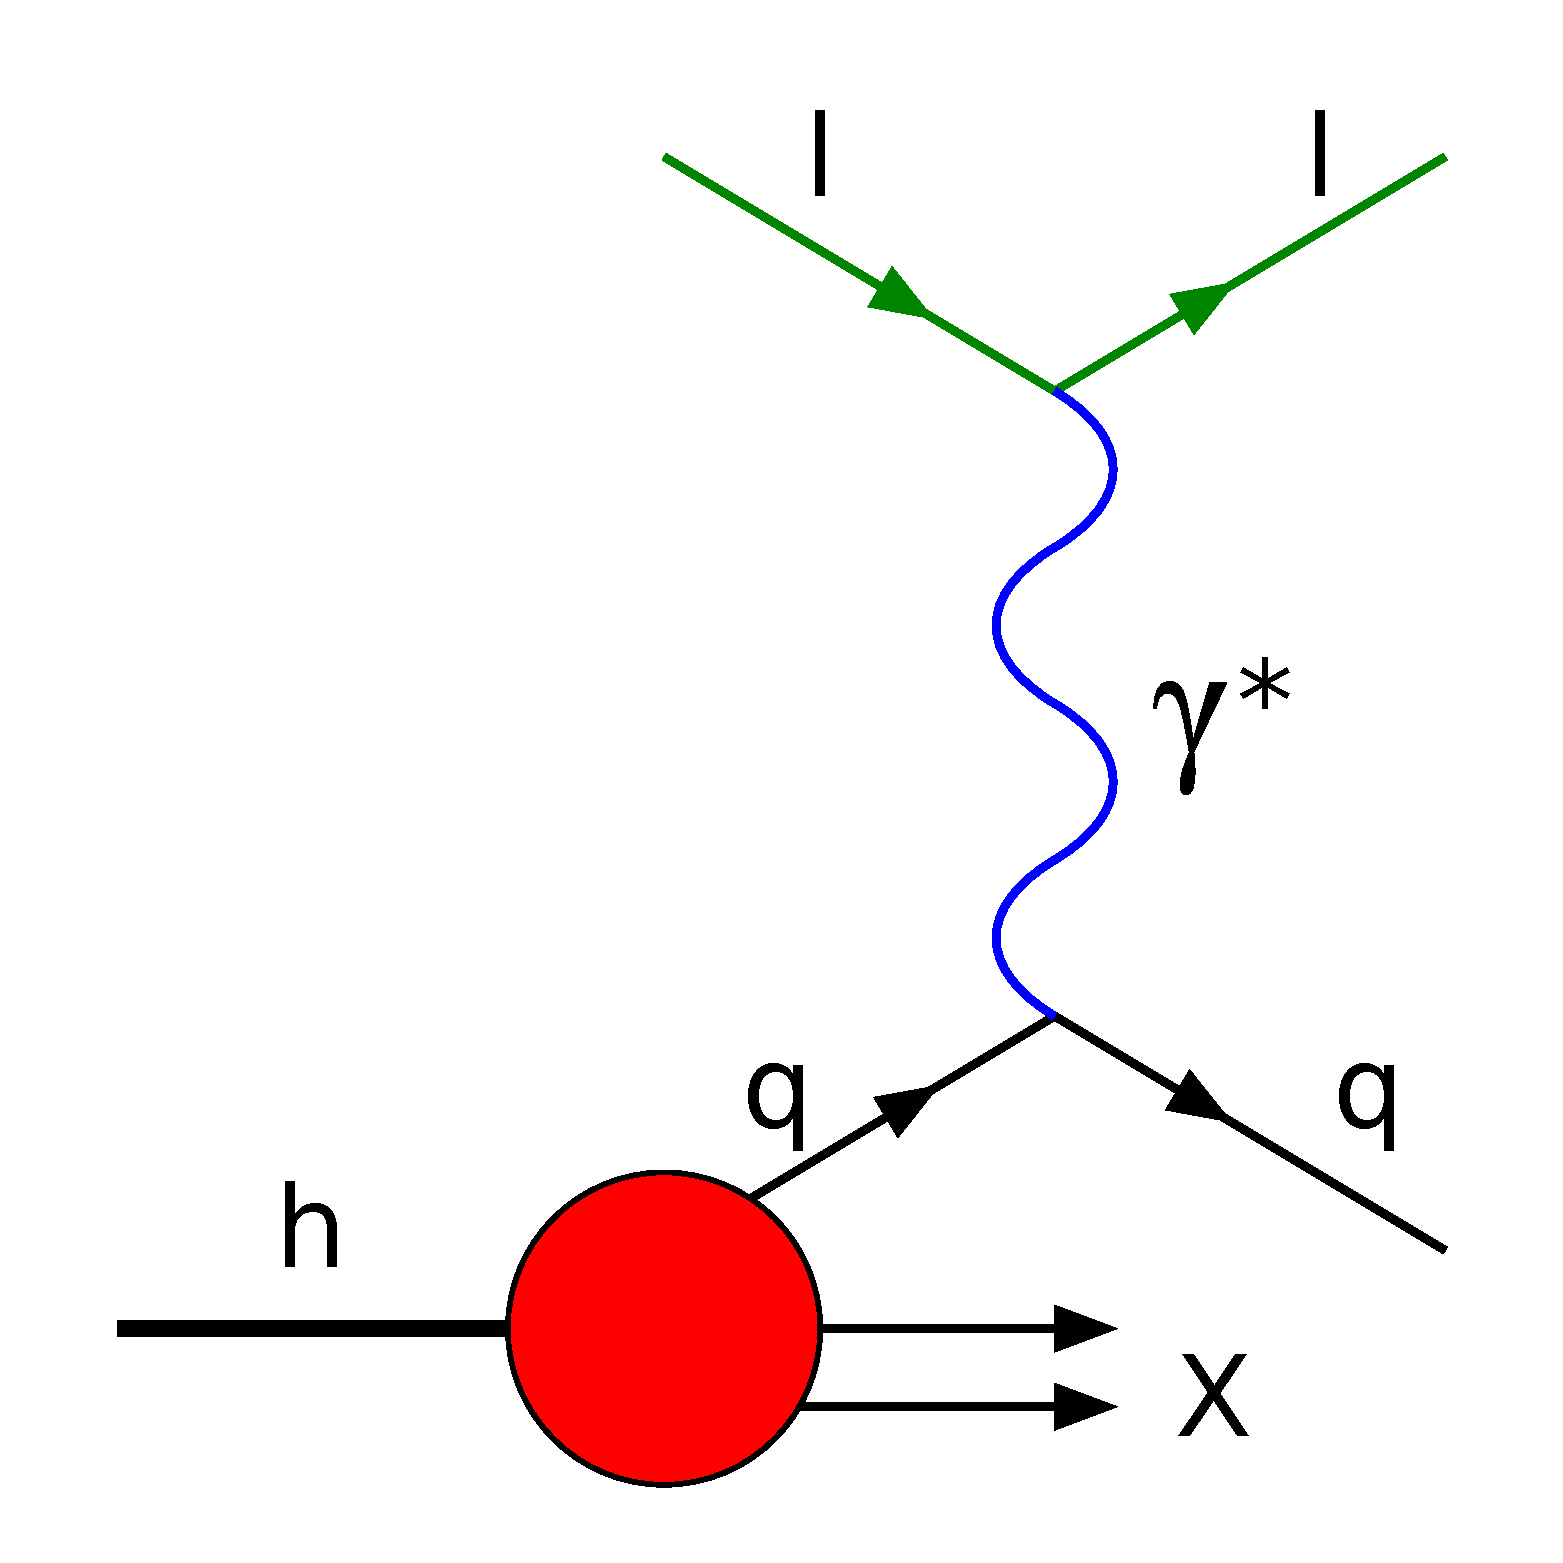
\includegraphics[width=0.3\linewidth]{DIS}
	\begin{tikzpicture}
	\tikzstyle{every node}=[font=\large]
	\begin{feynman}
		\vertex  (a1) {$l$};
		\vertex [right= 4cm of a1] (a2) {$l'$};

		\vertex [below= 4cm of a1,blob] (b2) {};
		\vertex [left= 1.2cm of b2] (b1) {$h$};
		\vertex[right= 2cm of b2] (b3){$X$};

		\vertex  at ($(a1) + (2cm , -1cm)$) [dot] (d);
		\vertex [below= 2 cm of d] (d1);

		\vertex at ($(d1) + (2cm, -1cm)$) (c1) {$q'$};
		
		\diagram*{
		(a1) --[fermion](d),
		(d)  --[fermion](a2),
		(b1) --[fermion](b2),
		(b2) --[fermion, edge label=$q$](d1),
		(d1) --[fermion](c1),
		(b2) --[double distance=4pt, thick](b3),
		(d) --[photon, edge label=$\gamma^*$](d1);
		};
	\end{feynman}
\end{tikzpicture}

	\caption{The Feynman diagram for DIS.}
	\label{fig:DIS}
\end{figure}
Similar to \cref{eq:ep_cs}, the DIS cross section can be expressed as
\begin{equation}
	\eval{\frac{d^2\sigma}{dE^\prime d\Omega}}_{DIS} = \frac{\alpha^2}{4E^2 \sin^4
		\frac{\theta}{2}} \left[ W_2\left(\nu,Q^2\right)\cos^2
		\frac{\theta}{2} + W_1\left(\nu,Q^2\right)\sin^2 \frac{\theta}{2}
		\right],
	\label{eq:DIS_cs1}
\end{equation}
where $\nu$ is the energy transferred by the scattering lepton.
In the elastic scattering, the cross section only depends on the momentum transfer squared $Q^2$,
as the energy transfer in $\nu$ is related to momentum transfer by $Q^2=2M\nu$.
In DIS, this relation no longer holds and the cross section would also depends on $\nu$.

It is also customary to define the structure functions $F_{1,2}$ from $W_{1,2}$ as:
\begin{equation}
	\begin{split}
		F_1\left(x,Q^2\right) & = MW_1\left(\nu,Q^2\right),    \\
		F_2\left(x,Q^2\right) & = \nu W_2\left(\nu,Q^2\right),
	\end{split}
\end{equation}
where $x=Q^2/2M\nu$ and $M$ is the mass of the nucleon. It was observed that at sufficiently high $Q^2$,
these structure functions $F_{1,2}$ are independent of $Q^2$, as illustrated in
\cref{fig:w2}. \Cref{fig:w2} shows the early measurements of the
structure function $F_2=\nu W_2$ as a function of $Q^2$ for a fixed
$x=1/\omega=0.25$ taken from Ref.~\cite{friedman1972}. This observation is
known as Bjorken scaling \cite{bjorken1969}.
\begin{figure}[htpb!]
	\centering
	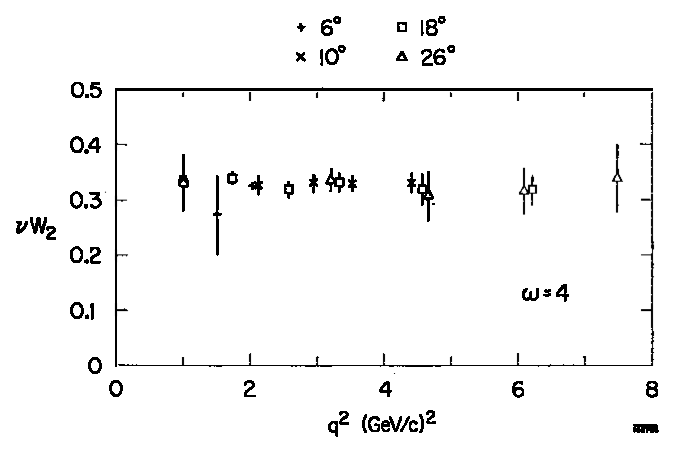
\includegraphics[width=0.5\linewidth]{nu_W2}
	\caption{Early measurement of the structure function $F_2=\nu W_2$ from
		fixed-target electron-proton deep inelastic scattering at SLAC for
		$x=1/\omega=0.25$, taken from Ref.~\cite{friedman1972}. The observation
		that $F_2(x,Q^2)$ is independent of $Q^2$ is known as Bjorken scaling. }
	\label{fig:w2}
\end{figure}
Taking the interpretation that the structure functions are related to the form factors in elastic scattering,
and therefore the Fourier transform of the charge distribution, the Bjorken scaling would suggest
the existence of point-like particles in the proton.

\section{Parton Model}
\label{sec:parton}
To explain the scaling behavior, Feynman proposed the parton model~\cite{feynman1969}.
In this model, hadrons are treated as extended objects which are made up of point-like
constituents (partons) held together by their mutual interaction. We now know
these partons are quarks and gluons described by QCD, but this was not known at
the time. Consider the DIS process, the hadron is Lorentz contracted in the
direction of the collision in the center-of-mass frame, and the internal
interaction are time dilated. As the center-of-mass energy increases, the
lifetime of the virtual partonic state is lengthened, and the time for the
electron to pass through the hadron is shortened. If the lifetime of the virtual
partonic states is longer than the duration of the electron-hadron interaction,
the partons are essentially frozen and the parton-parton interactions are
negligible. The hadrons can be considered as a collection of ``free'' partons,
and each parton may be thought of as carrying a certain fraction $x$ of the
hadron's momentum. The high energy lepton in DIS can be treated as scattering
off these partons elastically. The electron-parton elastic scattering can be
calculated using perturbative QCD, whereas the non-perturbative long-range
interaction within the hadron is encapsulated in the Parton Distribution
Function (PDF) $f_{a/h}\left(x\right)$, which can be interpreted as the probability
of finding a parton of species $a$ in hadron $h$ with fraction $x$ of the hadron's momentum.
And the cross section can be written as a convolution
of the non-perturbative PDF and the perturbative short range interaction. To leading
order (LO), the structure function $F_2\left(x,Q^2\right)$ is given by
\begin{equation}
	F_2\left(x,Q^2\right)=x\sum_i e^2_i f_{i/h}\left(x,Q^2\right),
	\label{eq:F2_parton}
\end{equation}
where $e_i$ is the charge carried by the quark and antiquark of flavor $i$. Since the
gluon does not carry any charge, it does not enter the cross section at leading
order. The ability to write the structure function and the cross section as a
convolution of the non-perturbative PDF and perturbative short range interaction
is known as the factorization theorem~\cite{collins1989}. These PDFs are also
expected to be universal and independent of the details of the scattering
process, as they describe the dynamics of the partons in a given hadron.

In the parton model, the structure functions $F_2$ and $F_1$ are clearly related. And
from \cref{eq:DIS_cs1}, the structure function $F_1$ is
related to the magnetic form factor $G_M$ in \cref{eq:ep_cs}. If the partons
are spin 0 particles, one would expect $F_1$ to be zero. In leading order of QCD,
only the quarks and antiquarks contribute to the cross section. Since quarks and
antiquarks are spin 1/2 particles, $F_1$ and $F_2$ are expected to satisfy the Callan-Gross
relation~\cite{callan1968,callan1969}
\begin{equation}
	F_2\left(x,Q^2\right) = 2x F_1\left(x,Q^2\right).
	\label{eq:CS_relation}
\end{equation}
The measured deviation from the Callan-Gross relation, defined as
\begin{equation}
	K_0 = \frac{F_2}{2xF_1}-1,
\end{equation}
is shown in \cref{fig:callan_gross}, taken from Ref.~\cite{kendall1991}.
For large $Q^2$, $K_0$ is consistent with zero, establishing the spin of the
charged partons is 1/2.
The deviation at low $Q^2$ is expected from the QCD corrections and contributions from
the gluons.
\begin{figure}[htbp!]
	\centering
	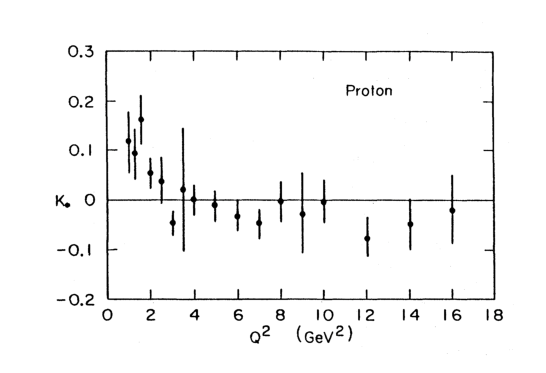
\includegraphics[width=0.5\linewidth]{Callan_Gross_relation}
	\caption{The deviation from the Callan-Gross relation, defined as
		$K_0=F_2/2xF_1 -1$, taken from Ref.~\cite{kendall1991}. This result
		demonstrates the spin 1/2 nature of the partons.}
	\label{fig:callan_gross}
\end{figure}

\section{Sum Rules}
\label{sec:sum_rules}
Since hadrons are characterized by their quantum numbers, hadrons consist of partons,
these quantum numbers serve as constraints on these PDFs.
For example, from the number of valence quarks in the proton,
one can impose the following constraints
\begin{equation}
	\begin{split}
		\int_{0}^{1} \dd{x} \left[f_{u/p} \left(x\right)-f_{\bar{u}/p} \left(x\right)\right] & =2,                                          \\
		\int_{0}^{1} \dd{x} \left[f_{d/p} \left(x\right)-f_{\bar{d}/p} \left(x\right)\right] & =1,                                          \\
		\int_{0}^{1} \dd{x} \left[f_{i/p} \left(x\right)-f_{\bar{i}/p} \left(x\right)\right] & =0 \qquad \text{for other quark flavors } i.
	\end{split}
\end{equation}
And the momentum of the hadron should be shared among the partons, hence
\begin{equation}
	\sum_{i=u,d,s,\cdots} \int_{0}^{1}\dd{x}\left[x f_{i/p}\left(x\right) +x f_{\bar{i}/p}\left(x\right) \right] + \int_{0}^{1}\dd{x} x f_{g/p}\left(x\right)=1
\end{equation}
An important sum rule is the Gottfried sum rule~\cite{gottfried1967}. It can be obtained
by using the charge symmetry,
which is the invariance under $u\leftrightarrow d$ and $\bar{u}\leftrightarrow \bar{d}$ interchange,
to relate the neutron distributions to those of
the proton, namely
\begin{equation}
	\begin{split}
		\bar{u}(x) \equiv f_{\bar{u}/p}(x) = f_{\bar{d}/n}(x); & \quad u(x) \equiv f_{u/p}(x) = f_{d/n}(x); \\
		\bar{d}(x) \equiv f_{\bar{d}/p}(x) = f_{\bar{u}/n}(x); & \quad d(x) \equiv f_{d/p}(x) = f_{u/n}(x).
	\end{split}
\end{equation}
The other quarks flavors and gluon distribution would be the same in both proton and neutron.
Using these relations and \cref{eq:F2_parton}, one obtains
\begin{equation}
	\begin{split}
		S_G & = \int_0^1 \frac{\dd{x}}{x}\left(F_2^{p}(x) - F_{2}^{n}(x)\right)                                     \\
		    & = \frac{1}{3} \int_0^1 \dd{x} \left[u\left(x\right) - d\left(x\right)
		+ \bar{u}\left(x\right) - \bar{d}\left(x\right)\right]                                                      \\
		    & = \frac{1}{3} \int_0^1 \dd{x} \left[u\left(x\right) - \bar{u}\left(x\right)\right]
		- \frac{1}{3} \int_0^1 \dd{x} \left[d\left(x\right) - \bar{d}\left(x\right)\right]
		+ \frac{2}{3} \int_0^1 \dd{x} \left[\bar{u}\left(x\right)-\bar{d}\left(x\right)\right]                      \\
		    & = \frac{1}{3} + \frac{2}{3} \int_0^1 \dd{x} \left[\bar{u}\left(x\right)-\bar{d}\left(x\right)\right].
	\end{split}
\end{equation}
If one assumes that $\bar{u}\left(x\right)= \bar{d}\left(x\right)$,
then $S_G$ would be $1/3$. This assumption can be tested using DIS.
One of the early measurements is from the New Muon Collaboration (NMC)~\cite{amaudruz1991}.
The $F_2^p-F_2^n$ measured by NMC is shown in \cref{fig:NMC_Gottfried}.
\begin{figure}[htbp!]
	\centering
	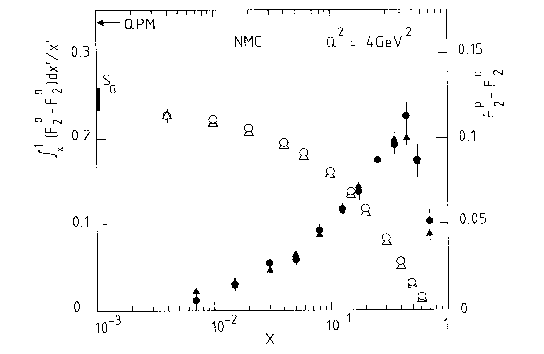
\includegraphics[width=0.7\linewidth]{Gottfried}
	\caption{The difference $F_2^p -F_2^n$ (solid and scale to the right) and
		$\int_{x_{min}}^1 (F_2^p-F_2^n)\dd{x}/x$ (open and scale to the left)
		determined by NMC, taken from Ref.~\cite{amaudruz1991}. The extrapolation
		to $x_{min}=0$ is indicated by the bar on the left vertical axis.}
	\label{fig:NMC_Gottfried}
\end{figure}
The extracted Gottfried sum is $0.240 \pm 0.016$, which is significantly below
$1/3$, suggesting an asymmetry in the light sea-quarks, $\bar{d}(x)\neq \bar{u}(x)$.

\section{Quantum Chromodynamics}
\label{sec:QCD}
\pdfmargincomment{General QCD}
Quantum Chromodynamics (QCD) is a theory of the strong interaction. It was
introduced by Fritzsch and Gell-Mann~\cite{fritzsch1972} and Fritzsch, Gell-Mann,
and Leutwyler~\cite{fritzsch1973}. QCD is a non-abelian gauge theory with an
$SU(3)$ gauge symmetry applied to the color degree of freedom. The $SU(3)$ group
chosen to account for (a) meson states made up of $q\bar{q}$ but not $qq$ bound states.
(b) There must be color singlet states. (c) The number of colors for each flavor
must be in agreement with the measured hadronic cross-section in $e^+ e^-$ collision.

An important feature of QCD is the asymptotic freedom. Being a renormalizable
theory, a regularization procedure and a set of renormalization prescription
need to be specified. In the renormalization process, the renormalized coupling $\alpha(\mu)$
is introduced and this coupling would be a function of the renormalization scale $\mu$.
It is noted that the coupling constant vanishes as $Q/\mu$ tends to infinity~\cite{gross1973,politzer1973},
allowing perturbative expansion of QCD at large $Q$.


\subsection{QCD Improved Parton Model and Scaling Violation}
\label{subsec:scaling_violation}
In QCD, the parton distribution functions can be defined as matrix elements of
operators acting on the hadron state. These operators act to count the number of
quarks and gluons carrying a fraction $\xi$ of the hadron's momentum. For quarks,
the distribution is given by~\cite{collins1989}
\begin{equation}
	f_{q/h}\left(\xi\right) = \frac{1}{4\pi}\int \dd{x} e^{-i\xi P^{+} x^{-}} \mel{P}{\bar{\psi}\left(0,x^-,0_\perp\right)\gamma^+ \mathcal{G} \psi\left(0,0,0_\perp\right)}{P},
\end{equation}
where $\mathcal{G}$ is the gauge link operator
\begin{equation}
	\mathcal{G}=\mathcal{P} \exp \left\{ ig\int_0^{x^-}\dd{y^-} A_c^+ \left(0,y^-,0_\perp\right)t_c\right\},
\end{equation}
where $\mathcal{P}$ denoted the path ordering of the gluon field operators $A_c^+$
along the path. Similarly, the gluon distribution function is given by
\begin{equation}
	f_{g/h}\left(\xi\right) = \frac{1}{2\pi\xi P^+}\int \dd{x} e^{-i\xi P^{+} x^{-}} \mel{P}{\tensor{F_a\left(0,x^-,0_\perp\right)}{^+^\nu} \tensor{\mathcal{G}}{_a_b} \tensor{F_b\left(0,0,0_\perp\right)}{_\nu^+}}{P},
\end{equation}
where $F^a_{\mu\nu}$ is the field tensor operator, and the octet representation of the $SU(3)$
generating matrices $t_c$ is used in $\mathcal{G}$.

The QCD generalization of \cref{eq:F2_parton} is
\begin{equation}
	\frac{1}{x}F_2\left(x,Q^2\right) = \sum_a \int_x^1 \frac{\dd{\xi}}{x}f_{a/h}\left(\xi,\mu\right)\frac{\xi}{x}H_{2a}\left( \frac{x}{\xi}, \frac{Q}{\mu}, \alpha_s\left(\mu\right)\right)
	+ \text{Remainder}.
\end{equation}
The hard scattering coefficient $H_{2a}$ is expanded as power series in $\alpha_s$. It
can be shown that the remainder is suppressed by powers of $Q$. Here the parton
distribution also depends on the renormalization scale $\mu$. This scale
dependency is introduced by the renormalization procedure. By requiring the cross
section and the structure functions to be independent of the scale $\mu$,
one can show that the renormalization group equation for the distribution
functions is
\begin{equation}
	\mu\frac{d}{d\mu}f_{a/h}\left(\xi,\mu\right)=\sum_b \int_\xi^1 \frac{\dd{\zeta}}{\zeta} P_{a/b}\left(\zeta,\alpha_s\left(\mu\right)\right) f_{b/h}\left(\frac{\xi}{\zeta},\mu\right),
\end{equation}
where $P_{a/b}$ is the Altarelli-Parisi kernel~\cite{altarelli1977}.

At order $\alpha_s$, the $F_2$ structure function is given by~\cite{collins1989}
\begin{equation}
	\frac{1}{x} F_2\left(x,Q^2\right) = \sum_j e^2_j f_{j/h}\left(x,\mu\right) + \sum_{j,b} e^2_j \int^1_x \frac{\dd{\xi}}{\xi} f_{b/h}\left(\xi,\mu\right) \frac{\alpha_s}{\pi} C_{jb}\left(\frac{x}{\xi}, \frac{Q}{\mu}\right) + \mathcal{O}(\alpha_s^2).
\end{equation}
The sum over $j$ runs over the quark and antiquark flavors. While the gluons
did not contribute at leading order, they contribute at order $\alpha_s$ through
virtual quark-antiquark pairs. The hard scattering coefficients $C_{jb}$ are
given by
\begin{align}
	C_{jk}(z,1) & = \delta_{jk} \frac{4}{3} \left[ -\frac{1}{2}\frac{1+z^2}{1-z} \ln\left(\frac{z}{1-z}\right) + \frac{3}{4} \frac{1}{1-z} -\frac{3}{2} -z\right]_+ \\
	C_{jg}(z,1) & = -\frac{1}{2} \left\{ \frac{1}{2}\left[z^2+(1-z)^2\right] \left[\ln\left(\frac{z}{1-z}\right)+1\right] -3z(1-z)\right\},
\end{align}
where the plus subscript denotes the subtraction that regulates the $z\rightarrow1$
singularity,
\begin{equation}
	\begin{split}
		\int^1_x \dd{z} \left[C(z)\right]_+ h(z) & = \int_0^1 \dd{z} \left[C(z)\right]_+ h(z)\Theta(z>x)        \\
		                                         & = \int_0^1 \dd{z} C(z) \left\{h(z)\Theta(z>x) -h(1)\right\}.
	\end{split}
\end{equation}

It is customary to choose $\mu =Q$ to avoid large logarithms of $\mu /Q$ in the
power expansions of $H$. As such the $\mu$ dependency in the parton distribution
functions can be interpreted as a virtual photon with higher $Q$ would probe the
nucleon with better resolution.

\Cref{fig:DIS_scaling} shows the extracted $F_2$ from DIS measurements compared
with the NLO calculation. The $Q^2$ dependency is known as scaling violation and
originates from higher order corrections and $Q$ dependency of the PDF.
\begin{figure}[h!]
	\centering
	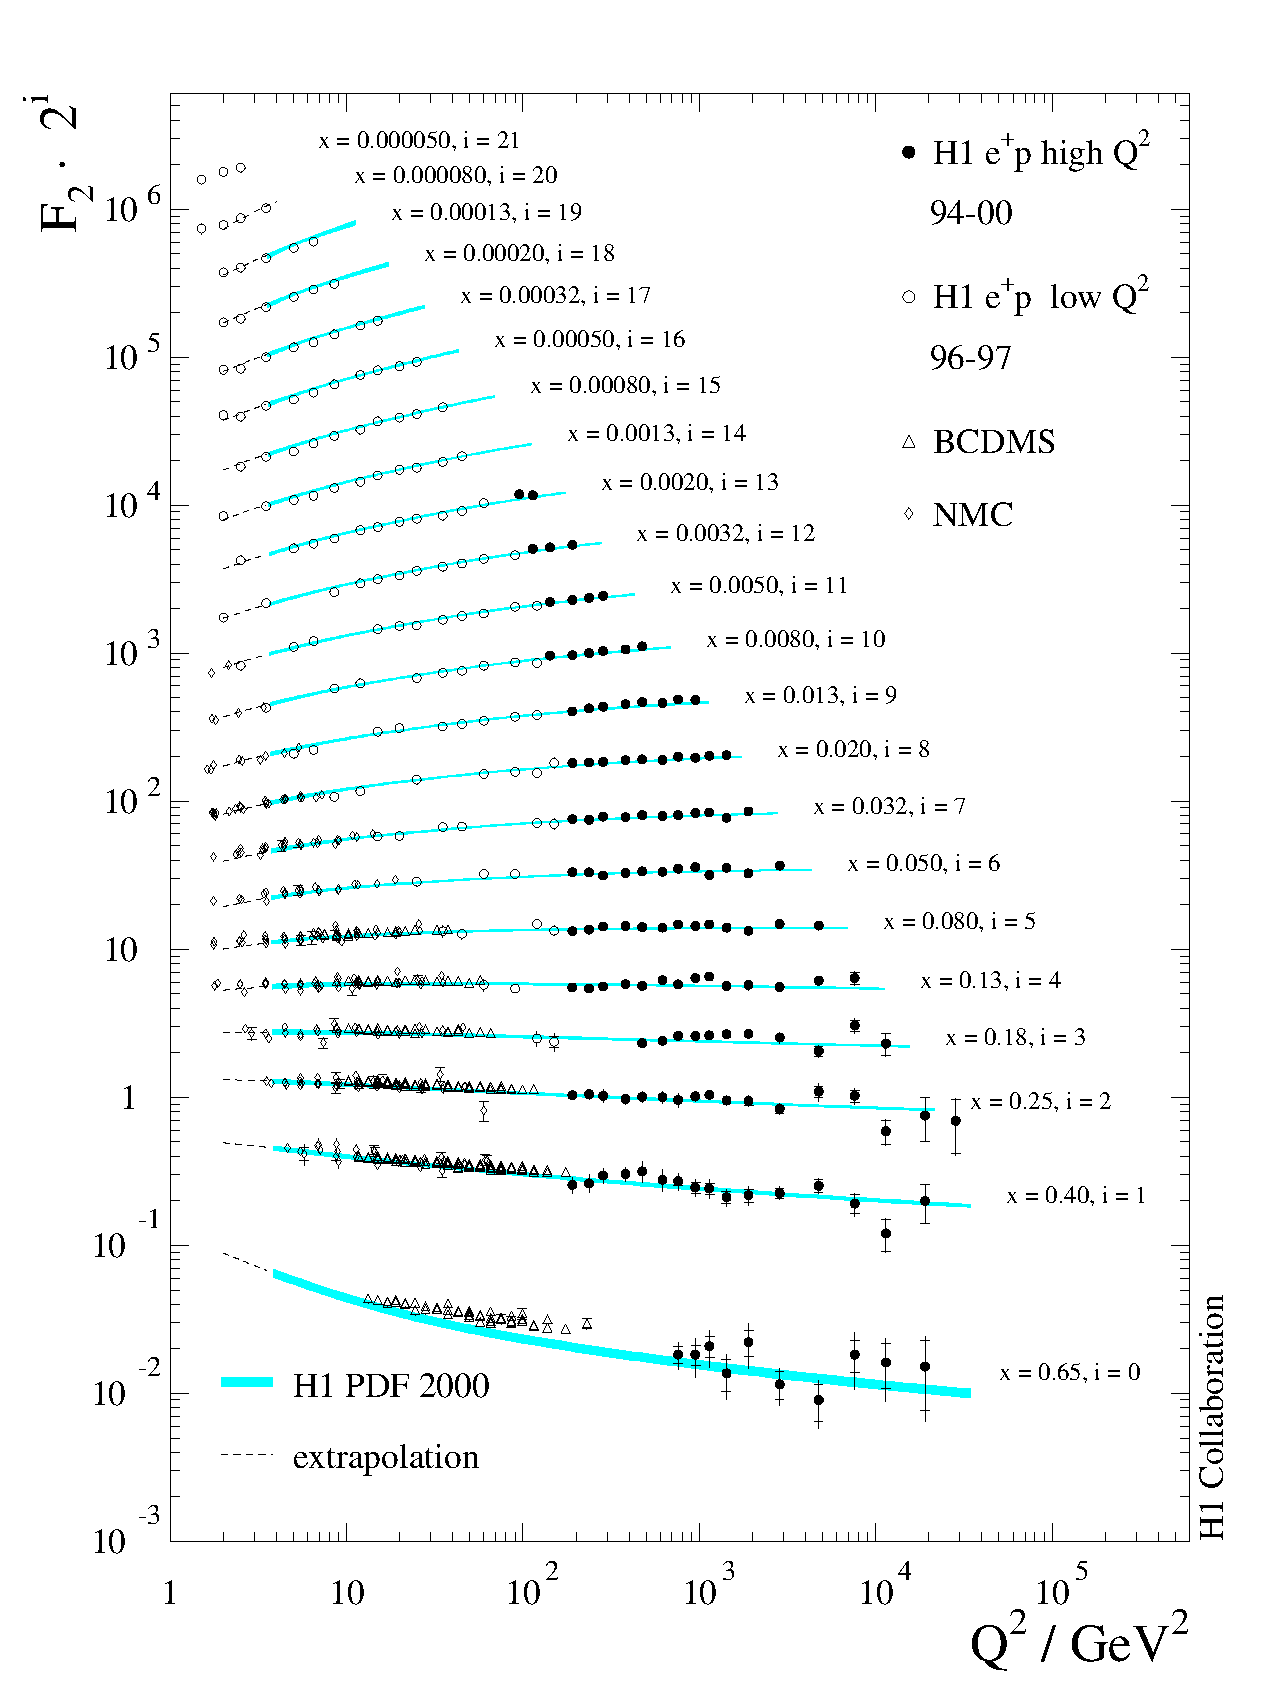
\includegraphics[width=0.6\linewidth]{DIS_scaling}
	\caption{
		Compilation of data on DIS, and compared with NLO calculations,
		taken from Ref.~\cite{adloff2003}.
		The $Q^2$ dependency is known as scaling violation,
		and originates from higher order corrections and $Q$ dependency of the PDF.
	}
	\label{fig:DIS_scaling}
\end{figure}
The Gottfried Sum Rule introduced in \cref{sec:sum_rules} would also be modified due to
QCD effects. At order $\alpha_s^2$, in the limit of a symmetric sea, the Gottfried Sum Rule
is given by~\cite{kataev2003}
\begin{equation}
	I_{GSR} = \begin{cases}
		\frac{1}{3}\left[ 1 + 0.0355\left(\frac{\alpha_s}{\pi}\right)-0.811\left(\frac{\alpha_s}{\pi}\right)^2 \right] & n_f=3, \\
		\frac{1}{3}\left[ 1 + 0.0384\left(\frac{\alpha_s}{\pi}\right)-0.822\left(\frac{\alpha_s}{\pi}\right)^2 \right] & n_f=4,
	\end{cases}
\end{equation}
where $n_f$ is the active flavor.
Taking $\alpha_s(Q^2=\SI{4}{\GeV^2})\approx 0.35$, the numerical value is $\approx 0.3313$. Therefore,
the light sea-quark asymmetry is still needed to explain the NMC result.

\Cref{fig:CT18_scale} shows the PDF extracted by CTEQ-TEA collaboration in their
CT18 global analysis~\cite{hou2021}. The sea-quarks from the gluon splitting
can be seen at low $x$ and is more important at large $Q$. This demonstrate the
QCD evolution of the PDF.

\begin{figure}
	\centering
	\begin{subfigure}{0.48\linewidth}
		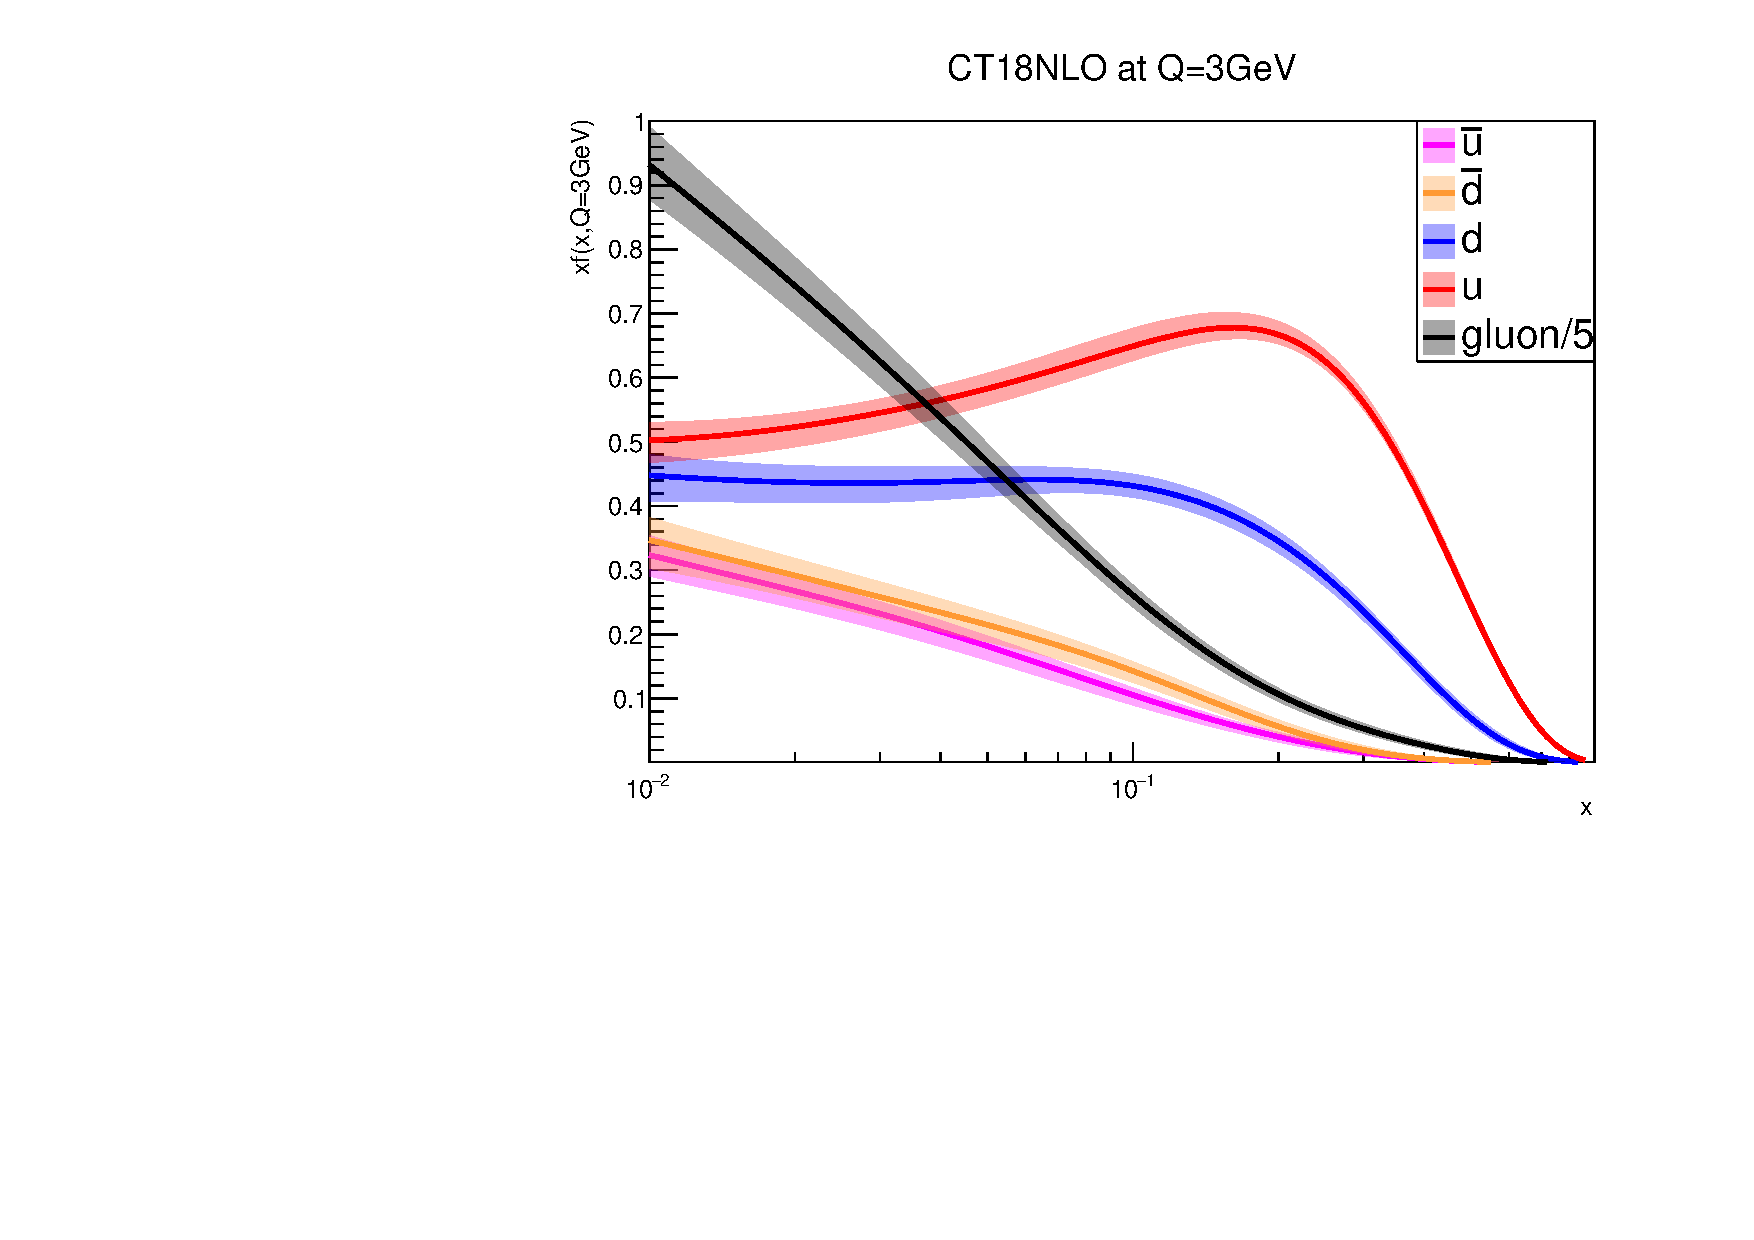
\includegraphics[width=\linewidth]{CT18NLO}
	\end{subfigure}
	\begin{subfigure}{0.48\linewidth}
		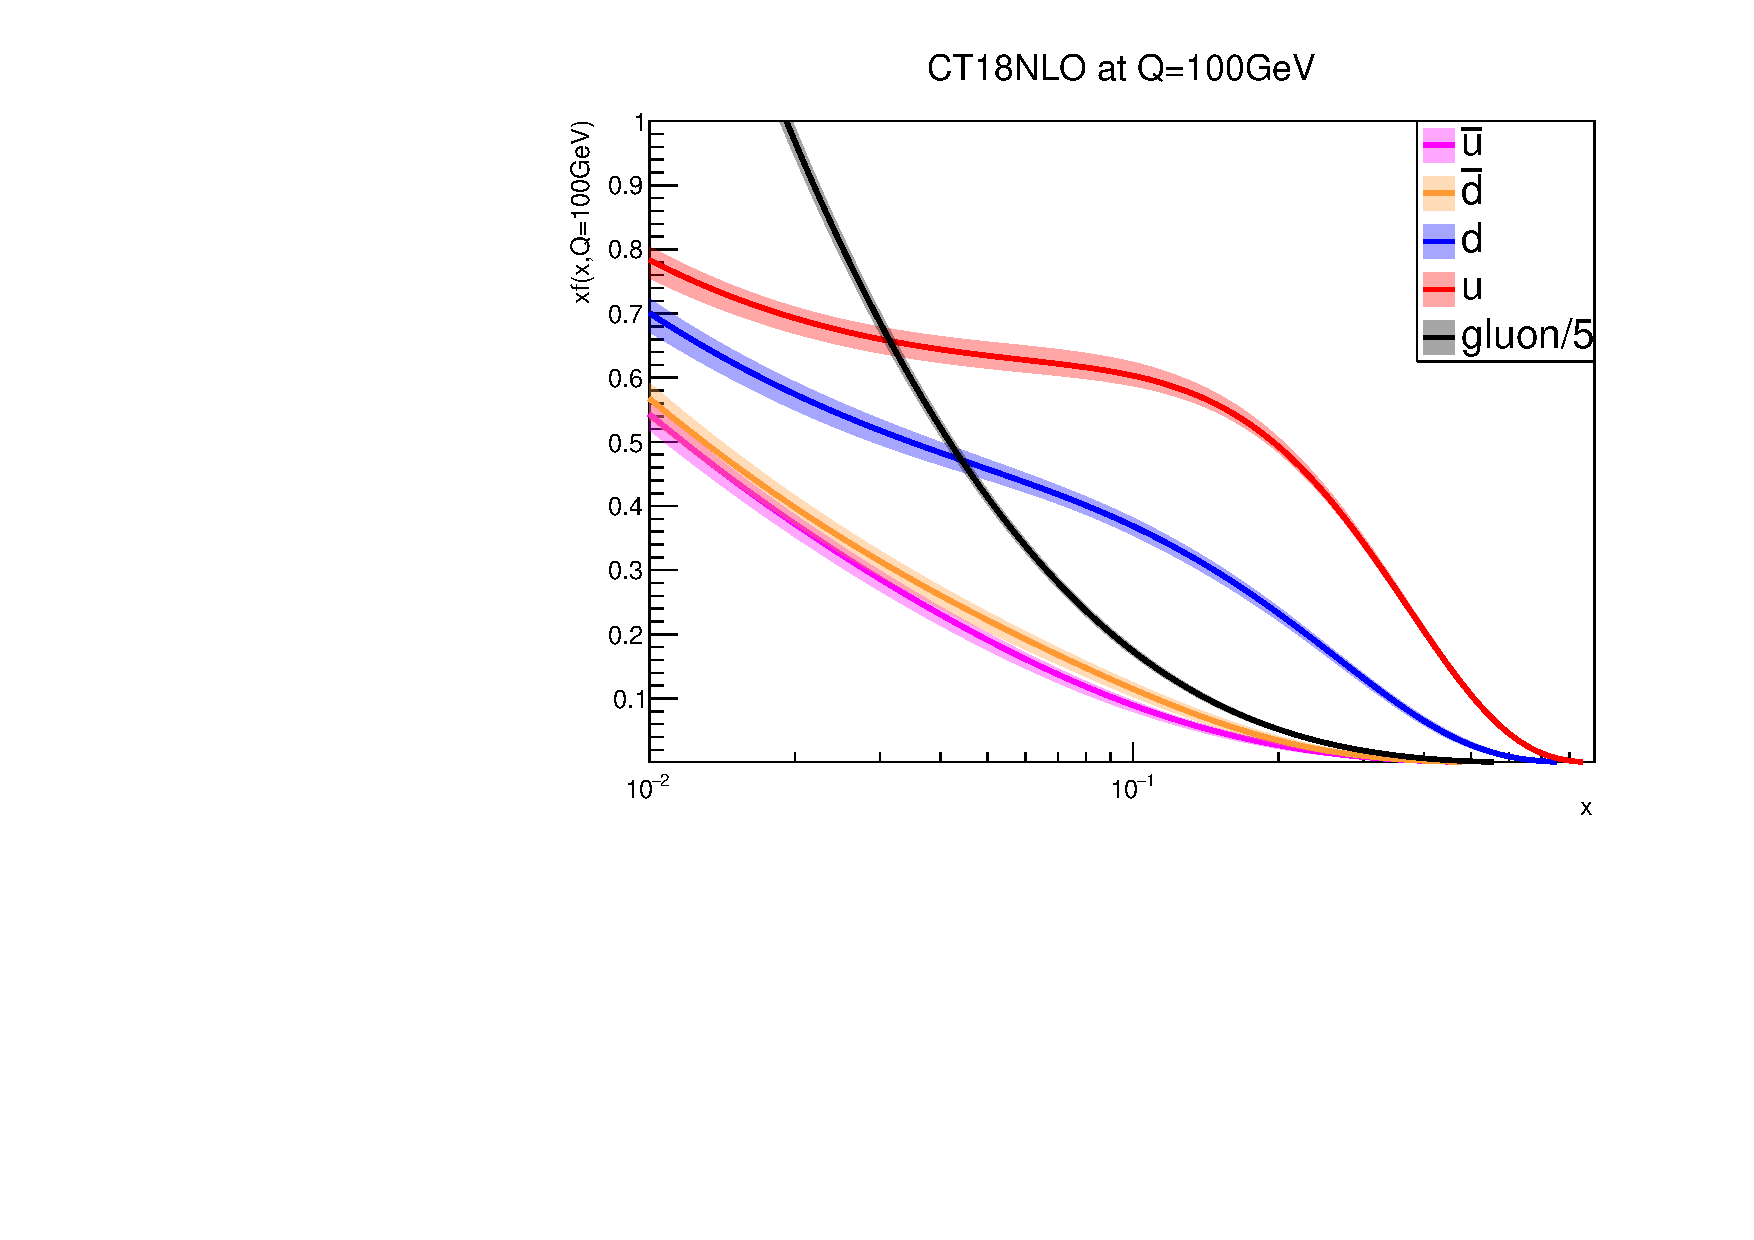
\includegraphics[width=\linewidth]{CT18NLO_100}
	\end{subfigure}
	\caption{The parton distribution functions from CT18~\cite{hou2021} global analysis at two different scales.
		The gluon distribution is scaled down by a factor of 5.}
	\label{fig:CT18_scale}
\end{figure}


\chapter{Drell-Yan Process}
\label{ch:DY}
In addition to DIS, another process for probing the hadron structure is the Drell-Yan process~\cite{drell1970}.
As illustrated in \cref{fig:DY}, this process involves two partons from the
two colliding hadrons to annihilate and form a lepton pair:
\begin{equation}
	h_A + h_B \rightarrow l + \bar{l} + X.
\end{equation}
The Drell-Yan process is related to the DIS process via crossing symmetry.
\begin{figure}[htbp!]
	\centering
	%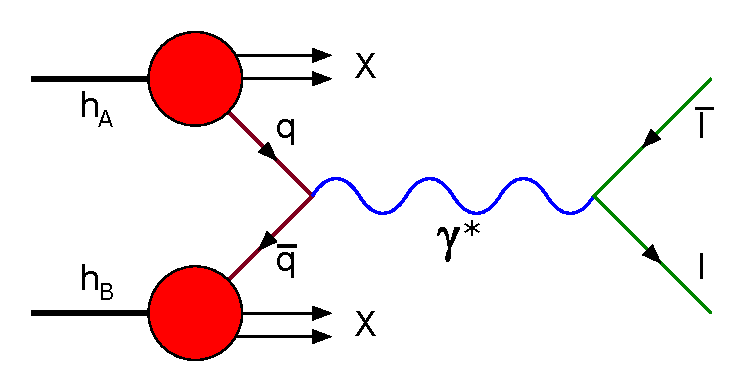
\includegraphics[width=0.5\linewidth]{Drell-Yan}
	\begin{tikzpicture}
	\tikzstyle{every node}=[font=\large]
	\begin{feynman}
		\vertex  (a1) {$h_A$};
		\vertex [right= of a1, blob] (a2) {};
		\vertex [right= 2cm of a2] (a3) {$X$};
		\vertex [below= 3cm of a1] (b1) {$h_B$};
		\vertex [below= 3cm of a2,blob] (b2) {};
		\vertex[below= 3cm of a3] (b3) {$X$};
		\vertex  at ($(b2) + (1.5cm , +1.5cm)$) [dot] (d);
		\vertex [right= 2.5 cm of d] (d1);
		\vertex at ($(d1) + (1.5cm , +1.2cm)$) (c1) {$l$};
		\vertex at ($(d1) + (1.5cm , -1.2cm)$) (c2) {$\bar{l}$};
		\diagram*{
		(a1) --[fermion](a2),
		(a2) --[double distance=4pt, thick](a3),
		(b1) --[fermion](b2),
		(b2) --[double distance=4pt, thick](b3),
		(d) --[fermion, edge label=$\bar{q}$] (b2),
		(a2) --[fermion, edge label=$q$](d),
		(d) --[photon, edge label=$\gamma^*$](d1),
		(c2) --[fermion] (d1);
		(d1) --[fermion] (c1);
		};
	\end{feynman}
\end{tikzpicture}

	\caption{The leading order Feynman diagram for the Drell-Yan process.}
	\label{fig:DY}
\end{figure}
Similar to DIS, the Drell-Yan cross section can be factorized into the non-perturbative
PDF and the perturbative parton-parton scattering. And the proof of factorization
theorem for Drell-Yan can be found in Ref.~\cite{collins1989}. At leading-order,
the cross section can be written as
\begin{equation}
	\frac{d^2\sigma_{DY}}{dx_{1}dx_{2}} = \frac{4\pi\alpha^2}{9M^2}\sum_q e^2_q
	\left[f_{q/A}\left(x_1\right)f_{\bar{q}/B}\left(x_2\right) +
	f_{\bar{q}/A}\left(x_1\right)f_{q/B}\left(x_2\right)
	\right],
	\label{eq:DY_cs}
\end{equation}
where $M$ is the mass of the lepton pair, $x_1$ and $x_2$ are the momentum fractions
carried by the partons from the two colliding hadrons. To simplify the notation,
the $Q^2$ scale dependence of the PDF is omitted here. In fixed target environments,
the scale $Q^2$ is typically chosen to the dilepton mass squared $M^2$.
The mass of the lepton pair and momentum fractions are related through
\begin{equation}
	M^2= sx_1x_2,
	\label{eq:mass}
\end{equation}
where $s$ is the hadron-hadron center-of-mass energy squared.
Since the underlying mechanism for the Drell-Yan process at leading order involves the annihilation
of a quark and an antiquark, this process is particularly useful in probing the antiquark
content of the hadron.
In the parton model, the angular distribution of the Drell-Yan dilepton would have the following
distribution from the decay of the transversely polarized virtual photon,
\begin{equation}
	\dv{\sigma_{DY}}{\Omega} = \sigma_0(1+\lambda \cos^2\theta),
\end{equation}
where $\theta$ is the polar angle of the lepton in the virtual photon rest frame and $\lambda=1$.

The Drell-Yan process and the parton model has been successful in explaining the shape of
the dimuon production cross section and the angular distribution in early experiments. However,
the  experimental cross section was about a factor of two larger than predicted, and the
transverse momentum of the dilepton is larger than expected from the convolution of the intrinsic
parton momenta~\cite{mcgaughey1999}. These discrepancies can be resolved if higher order
QCD correction is included.
\begin{figure}[htbp!]
	\centering
	\begin{subfigure}{0.45\linewidth}
		\centering
		\begin{tikzpicture}
	\tikzstyle{every node}=[font=\large]
	\begin{feynman}
		\vertex  (a1){$q$};
		\vertex [right= 4cm of a1] (a2) {$\gamma^*$};
		\vertex [below= 4cm of a1] (b1) {$\bar{q}$};
		\vertex[below= 4cm of a2] (b2) {$g$};
		\vertex  at ($(a1) + (2cm , -1cm)$) [dot] (d);
		\vertex [below= 2 cm of d] (d1);
		\diagram*{
		(a1) --[fermion](d),
		(d1) --[fermion](b1),
		(d) --[fermion] (d1),
		(d1) --[gluon](b2),
		(d) --[photon](a2);
		};
	\end{feynman}
\end{tikzpicture}

		\caption{Gluon bremsstrahlung.}
		\label{subfig:DY_gb}
	\end{subfigure}
	\begin{subfigure}{0.45\linewidth}
		\centering
		\begin{tikzpicture}
	\tikzstyle{every node}=[font=\large]
	\begin{feynman}
		\vertex  (a1){$q$};
		\vertex at ($(a1) + (1cm, -1cm)$) (a2);
		\vertex [below= 4cm of a1] (b1) {$\bar{q}$};
		\vertex [below= 2 cm of a2] (b2);
		\vertex at ($(a2) + (1cm, -1cm)$) (d);
		\vertex [right= 2 cm of d] (d1){$\gamma^*$};
		\diagram*{
		(a1) --[fermion](a2),
		(b2) --[fermion](b1),
		(a2) --[gluon] (b2),
		(a2) --(d),
		(b2) --(d),
		(d) --[photon](d1);
		};
	\end{feynman}
\end{tikzpicture}

		\caption{Interference from $\mathcal{O}(\alpha^2_s)$.}
		\label{subfig:DY_interfer}
	\end{subfigure}

	\begin{subfigure}{\linewidth}
		\centering
		\begin{subfigure}{0.45\linewidth}
			\centering
			\begin{tikzpicture}
	\tikzstyle{every node}=[font=\large]
	\begin{feynman}
		\vertex  (a1){$q$};
		\vertex [right= 4cm of a1] (a2) {$q$};
		\vertex [below= 4cm of a1] (b1) {$g$};
		\vertex[below= 4cm of a2] (b2) {$\gamma^*$};
		\vertex  at ($(b1) + (1cm , +2cm)$) [dot] (d);
		\vertex [right= 2 cm of d] (d1);
		\diagram*{
		(a1) --[fermion](d),
		(b1) --[gluon](d),
		(d) --[fermion] (d1),
		(d1) --[fermion](a2),
		(d1) --[photon](b2);
		};
	\end{feynman}
\end{tikzpicture}

		\end{subfigure}
		\begin{subfigure}{0.45\linewidth}
			\centering
			\begin{tikzpicture}
	\tikzstyle{every node}=[font=\large]
	\begin{feynman}
		\vertex  (a1){$q$};
		\vertex [right= 4cm of a1] (a2) {$\gamma^*$};
		\vertex [below= 4cm of a1] (b1) {$g$};
		\vertex[below= 4cm of a2] (b2) {$q$};
		\vertex  at ($(a1) + (2cm , -1cm)$) [dot] (d);
		\vertex [below= 2 cm of d] (d1);
		\diagram*{
		(a1) --[fermion](d),
		(b1) --[gluon](d1),
		(d) --[fermion] (d1),
		(d1) --[fermion](b2),
		(d) --[photon](a2);
		};
	\end{feynman}
\end{tikzpicture}

		\end{subfigure}
		\caption{Gluon Compton scattering.}
		\label{subfig:DY_gc}
	\end{subfigure}
	\caption{Examples of diagrams contributing to the Drell-Yan cross section
		at NLO.}
	\label{fig:NLO_DY}
\end{figure}
At NLO ($\mathcal{O}\left(\alpha_s\right)$), diagrams such as gluon bremsstrahlung
and Compton scattering begin to contribute, as shown in \cref{fig:NLO_DY}.

The cross section for the annihilation process is given by the sum of the LO Drell-Yan expression and
the NLO correction~\cite{kubar1980}
\begin{equation}
	\frac{d^2\sigma^A}{dQ^2dx_{F}} = \sum_q e^2_q \int^1_{x_1} \dd{t_1} \int^1_{x_2} \dd{t_2}
	\left[ \frac{d^2\hat{\sigma}^{DY}}{dQ^2dx_F}+\frac{d^2\hat{\sigma}^{A}}{dQ^2dx_F} \right]
	\left[f_{q/A}\left(t_1\right)f_{\bar{q}/B}\left(t_2\right) +
	f_{\bar{q}/A}\left(t_1\right)f_{q/B}\left(t_2\right)
	\right].
\end{equation}
Where Feynman-$x$ ($x_F$) is typically given by the difference of $x_1$ and $x_2$ and is related to the
longitudinal momentum of the dimuon pair ($P_L$) in the hadron-hadron center-of-mass frame.
\begin{equation}
	x_F = x_1 - x_2 = \frac{2P_L}{\sqrt{s}}.
\end{equation}
The LO Drell-Yan term is given by
\begin{equation}
	\frac{ d^2\hat{\sigma}^{DY} }{dQ^2 dx_F} = \frac{4\pi\alpha^2}{9Q^2 s} \frac{1}{x_1+x_2}\delta\left(t_1-x_1\right)\delta\left(t_2-x_2\right).
\end{equation}
The NLO correction to the annihilation process, from \cref{subfig:DY_gb,subfig:DY_interfer},
is given by
\begin{equation}
\begin{split}
	\frac{d^2\hat{\sigma}^{A}}{dQ^2dx_F} =& \frac{1}{2}A \frac{\delta\left(t_1-x_1\right)\delta\left(t_2-x_2\right)}{\left(x_1+x_2\right)} \left[ 1+\frac{5}{3}\pi^2 - \frac{3}{2}\ln\frac{x_1x_2}{\left(1-x_1\right)\left(1-x_2\right)} + 2\ln\frac{x_1}{1-x_1}\ln\frac{x_2}{1-x_2}\right]\\
	&+\frac{1}{2} A \frac{\delta\left(t_2-x_2\right)}{\left(x_1+x_2\right)}\left[\frac{t_1^2+x_1^2}{t_1^2\left(t_1-x_1\right)_{+}} \ln\frac{\left(x_1+x_2\right)\left(1-x_2\right)}{x_2\left(t_1+x_2\right)} + \frac{3}{2\left(t_1-x_1\right)_{+}} -\frac{2}{t_1} - \frac{3x_1}{t_1^2}\right]\\
	&+\left(1\leftrightarrow 2\right) + \frac{1}{2} A \left[\frac{G^A\left(t_1,t_2\right)}{\left[\left(t_1-x_1\right)\left(t_2-x_2\right)\right]_{+}} +H^A\left(t_1,t_2\right)\right],
\end{split}
\end{equation}
where the function $G^A$ and $H^A$ are given by
\begin{align}
	G^A\left(t_1,t_2\right) &= \frac{\left(t_1+t_2\right)\left(\tau^2+\left(t_1t_2\right)^2\right)}{\left(t_1t_2\right)^2\left(t_1+x_2\right)\left(t_2+x_1\right)},\\
	H^A\left(t_1,t_2\right) &= \frac{-2}{t_1t_2\left(t_1+t_2\right)}.
\end{align}
And
\begin{equation}
	A=\frac{16\alpha^2\alpha_s}{27Q^2s}, \quad \tau=x_1x_2.
\end{equation}

Similarly, the cross section for the Compton scattering process (\cref{subfig:DY_gc}) is given by 
\begin{equation}
	\frac{d^2\sigma^C}{dQ^2dx_{F}} = \sum_q e^2_q \int^1_{x_1} \dd{t_1} \int^1_{x_2} \dd{t_2}
	\frac{d^2\hat{\sigma}^{C}}{dQ^2dx_F} f_{g/A}\left(t_1\right)
	\left[f_{q/B}\left(t_2\right) +f_{\bar{q}/B}\left(t_2\right) \right] + \left(1,A\leftrightarrow 2,B\right),
	\label{eq:compton_full}
\end{equation}
where the partonic cross section is given by
\begin{equation}
	\begin{split}
		\frac{d^2\hat{\sigma}^{C}}{dQ^2dx_F} =&\frac{3}{16} A \frac{\delta\left(t_2-x_2\right)}{\left(x_1+x_2\right)t_1^3}\left[ \left(x_1^2+\left(t_1-x_1\right)^2\right)\ln\frac{\left(x_1+x_2\right)\left(1-x_2\right)}{x_2\left(t_1+x_2\right)} - 6x_1\left(t_1-x_1\right)+t_1^2\right]\\
		&+\frac{3}{16}A\left[\frac{G^C\left(t_1,t_2\right)}{\left(t_2-x_2\right)_{+}} + H^C \left(t_1,t_2\right) \right],
	\end{split}
\end{equation}
and
\begin{align}
	G^C\left(t_1,t_2\right) &= \frac{\tau^2+\left(t_1t_2-\tau\right)^2}{t_1^3t_2^2\left(t_2+x_1\right)},\\
	H^C\left(t_1,t_2\right) &= \frac{1}{\left(t_1t_2\right)^2\left(t_1+t_2\right)^2}\left[t_1\left(t_2+x_1\right)\left(t_2-x_2\right)+2\tau\left(t_1+t_2\right)\right].
\end{align}
Note that in the second term of \cref{eq:compton_full}, the indices 1 and 2 must also be exchange in
the expression of $\flatfrac{d^2\hat{\sigma}^{C}}{dQ^2dx_F}$.



Including higher-order QCD corrections, the angular distribution for the Drell-Yan dilepton would
be modified as follows:
\begin{equation}
	\dv{\sigma_{DY}}{\Omega} \propto 1 + \lambda \cos^2\theta + \mu \sin 2\theta\cos\phi +\frac{\nu}{2}\sin^2\theta\cos 2\phi,
\end{equation}
where $\phi$ is the azimuthal angle. And the angle-independent parameters are expected to have the
following relation~\cite{lam1980}
\begin{equation}
	1-\lambda-2\nu=0.
\end{equation}
This relation, known as the Lam-Tung relation, is analogous to the Callan-Gross relation in DIS
(\cref{eq:CS_relation}).

\Cref{fig:DY_scaling} shows some of the existing data on Drell-Yan compared with NLO calculation. By
performing a global fit to both DIS and Drell-Yan data, the parton distribution
functions can be extracted. The ability to fit both DIS and Drell-Yan data using
the same PDF demonstrate the universality of the PDF and the validity of the
factorization theorem.
\begin{figure}[htbp!]
	\centering
	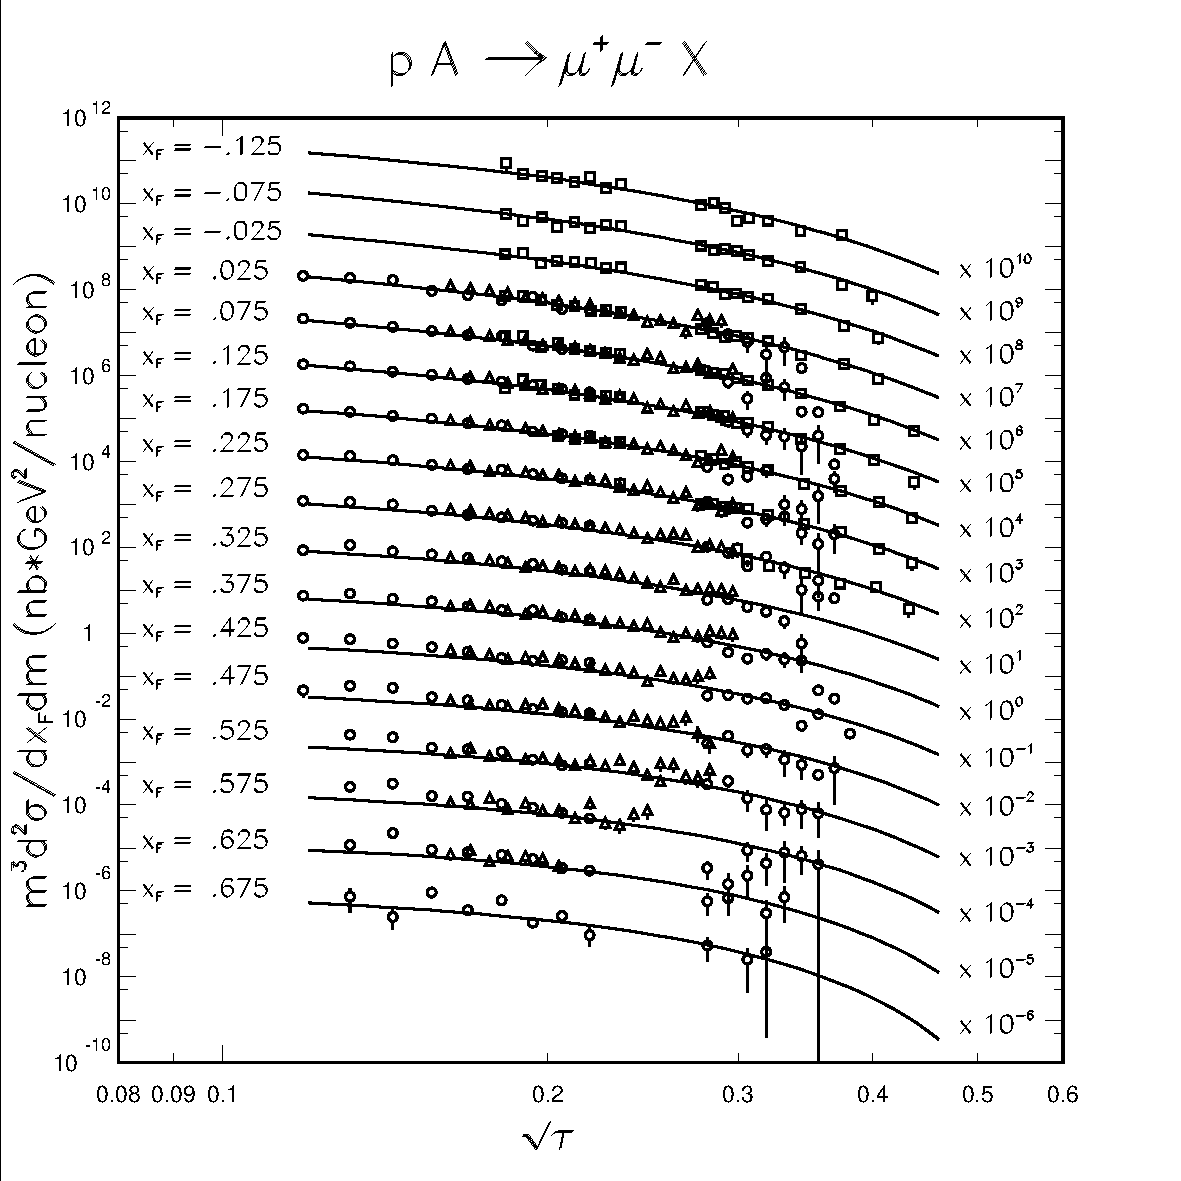
\includegraphics[width=0.8\linewidth]{DY_scaling}
	\caption{Compilation of data on Drell-Yan process, and compared with NLO calculations,
		taken from Ref.~\cite{mcgaughey1999}.}
	\label{fig:DY_scaling}
\end{figure}

One of the advantages of Drell-Yan over DIS is the explicit separation of the quark
and anti-quark distributions in \cref{eq:DY_cs}. At large $x$, DIS cross section
is dominated by the valence quark distribution. On the other hand, in the region $x_1 \gg x_2$,
the valence quark in the Drell-Yan process is more likely to come from the beam
hadron, and the anti-quark is more likely to come from the target hadron. Hence,
Drell-Yan can be more sensitive to the anti-quark distribution than DIS. In
particular, the $\sigma_{pd}/2\sigma_{pp}$ Drell-Yan cross section ratio at leading order
can be approximated as
\begin{equation}
	\frac{\sigma_{pd}}{2\sigma_{pp}}\approx \frac{\sigma_{pp}+\sigma_{pn}}{2\sigma_{pp}}
	\stackrel{x_1\gg x_2}{\approx} \frac{1}{2} \left( 1+ \frac{\frac{\bar{d}\left(x_2\right)}{\bar{u}\left(x_2\right)} + \frac{d\left(x_1\right)}{4u\left(x_1\right)} }{1+\frac{d\left(x_1\right)}{4u\left(x_1\right)} \frac{\bar{d}\left(x_2\right)}{\bar{u}\left(x_2\right)} }\right).
\end{equation}
The first approximation sign indicates that nuclear correction in deuteron is assumed to be negligible~\cite{ehlers2014}.
In the limit $x_1$ is sufficiently large, $d\left(x_1\right)/u\left(x_1\right)$ is expected
to be small, and thus this ratio can be directly related to the light sea-quark
asymmetry. The Drell-Yan process has been used in several experiments to probe the sea-quarks
asymmetry, with the goal of measuring the $x$ dependence of the sea-quark asymmetry
instead of only the integral as with the Gottfried sum rule.


\section{E866/NuSea}
\label{sec:E866}
Utilizing the sensitivity of the Drell-Yan process to the sea-quark asymmetry,
the E866/NuSea experiment~\cite{towell2001} was designed to measure the $\sigma_{pd}/2\sigma_{pp}$
Drell-Yan cross section ratio over a broad range of $x$. The
experiment utilized the \SI{800}{\GeV} proton beam from the Tevatron on liquid
hydrogen and deuterium targets. The measured deuterium over hydrogen cross section
ratio from E866/NuSea is shown in \cref{fig:e866_result}. At low $x$, the ratio is consistent
with a symmetric sea, and the asymmetry becomes larger as $x$ increases, as expected from
the model predictions. However, at $x_2>0.25$ the cross section ratios
drop below unity, suggesting that the $\bar{d}/\bar{u}$
ratio drop below 1, which could not be explained by models at the time.
Due to the large uncertainty on the data points at large $x_2$, a new
experiment was needed to explore sea quark asymmetry the high $x$ region with better
accuracy.
\begin{figure}[htbp!]
	\centering
	\begin{subfigure}{0.48\linewidth}
		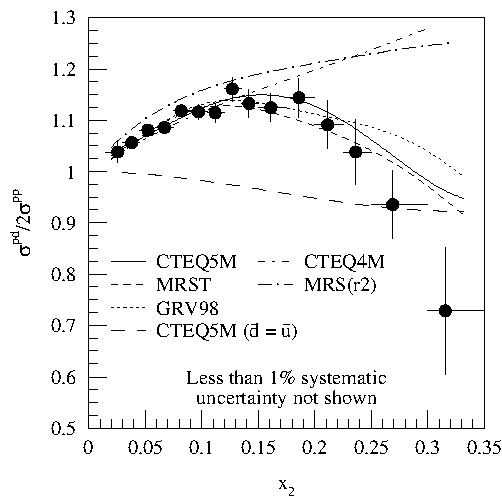
\includegraphics[width=\linewidth]{e866_csr}
		\caption{$\sigma_{pd}/2\sigma_{pp}$ Drell-Yan cross section ratio.}
		\label{subfig:e866_csr}
	\end{subfigure}
	\begin{subfigure}{0.48\linewidth}
		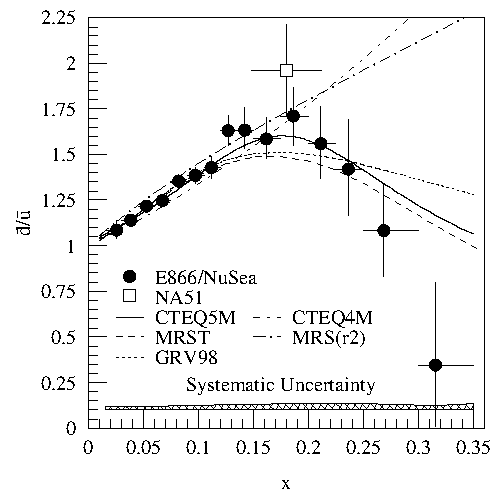
\includegraphics[width=\linewidth]{e866_dbarubar}
		\caption{$\bar{d}/\bar{u}$ extracted from E866 result.}
		\label{subfig:e866_dbarubar}
	\end{subfigure}
	\caption{The E866 result taken from Ref.~\cite{towell2001}.}
	\label{fig:e866_result}
\end{figure}

\section{Origin of the \texorpdfstring{$\bar{d}/\bar{u}$}{dbar/ubar} Asymmetry }
After the result from NMC and other DIS experiments indicating the violation of the Gottfried sum rule,
various models have been proposed to explain the $\bar{d}/\bar{u}$ asymmetry. One of the early proposal
is by Field and Feynman~\cite{field1977}. They suggested that the Pauli blocking effect
could suppress the production of $u\bar{u}$ pairs relative to  $d\bar{d}$ due to the presence of two
valence $u$ quarks and only one valence $d$ quark in the proton.
It was later shown that the effect by Pauli blocking would be small and
may actually have an opposite effect~\cite{steffens1997}. Since the contribution from gluon splitting to the
sea quarks is flavor-blind and the mass of $u$ and $d$ quarks are roughly equal, the asymmetry in the
light sea-quarks must originate from a non-perturbative mechanism. Some of the models will be presented
in this section.

\subsection{Meson Cloud Model}
Some of the early models attribute the asymmetry to the existence of a ``pion cloud'' in the proton.
In the meson cloud model~\cite{kumano1998,speth2002} the proton wave function is written as a sum of meson-baryon states
\begin{equation}
	\ket{p} = \sqrt{Z}\ket{p}_{\mathrm{bare}} + \sum_{MB}\int \dd{y} \dd[2]{\vec{k}_\perp} \phi_{BM} \left(y, k^2_\perp\right)\ket{M\left(y, \vec{k}_\perp\right);B\left(1-y, -\vec{k}_\perp\right)}
\end{equation}
where $\phi_{BM}$ is the amplitude to find a physical nucleon in a state consisting of a virtual
meson $M$ and virtual baryon $B$ with longitudinal momentum fractions $y$ and $1-y$ and transverse momenta
$\vec{k}_\perp$ and $-\vec{k}_\perp$ respectively. $Z$ is the standard wave function normalization factor
and can be interpreted as the probability of finding a bare proton, which only contains a symmetric sea and the valence quarks.

The main hypothesis is that the exchanged photon in the DIS process can interact with the partons in the
virtual meson or the virtual
baryon. Therefore, the PDF can be related to the PDFs of either the stuck meson or stuck baryon.
\begin{equation}
	f_{i/N}\left(x\right) = f_{i/N}^{\mathrm{bare}}\left(x\right) +  \int^1_x f_{MB/N}\left(y\right) f_{i/M}\left(\frac{x}{y}\right) \frac{\dd{y}}{y} + \int^1_x f_{BM/N}\left(y\right) f_{i/B}\left(\frac{x}{y}\right) \frac{\dd{y}}{y},
\end{equation}
where $f_{MB/N}$ and $f_{BM/N}$ are the splitting function, related to $\phi_{BM}$, and $f_{MB/N}(y)=f_{BM/N}(1-y)$.
If we restrict to $\pi N$ and $\pi\Delta$ states, and using isospin symmetry,
\begin{align}
	f_{\pi^+n/p}=\frac{2}{3} f_{\pi N}                                       & , ~f_{\pi^0 p/p}=\frac{1}{3} f_{\pi N},                                         \\
	f_{\pi^-\Delta^{++}/p}=\frac{1}{2} f_{\pi \Delta}, ~f_{\pi^0 \Delta^+/p} & =\frac{1}{3} f_{\pi \Delta},  ~f_{\pi^+ \Delta^0/p}=\frac{1}{6} f_{\pi \Delta}.
\end{align}
The light sea-quark distributions in the proton are given by
\begin{align}
	\bar{d}(x) & = \left(\frac{5}{6}f_{\pi N} + \frac{1}{3}f_{\pi \Delta}\right)\otimes q^v_\pi + S(x) \\
	\bar{u}(x) & = \left(\frac{1}{6}f_{\pi N} + \frac{2}{3}f_{\pi \Delta}\right)\otimes q^v_\pi + S(x)
	\label{eq:pion_dbub}
\end{align}
where $f\otimes q\equiv \int^1_x \frac{dy}{y}f(y)q\left(\frac{x}{y}\right)$, $q^v_\pi$ is the valence
quark distribution in pions, and $S(x)$ is the flavor symmetric contributions.
The asymmetry in the proton sea arises because of the dominance of the $\pi^+$ among the $\pi N$ states.
However, the effect is slightly reduced by the $\pi\Delta$ configurations, which favors $\bar{u}$ over $\bar{d}$.
As the $\Delta$ baryon is heavier than the proton, the $\pi\Delta$ configurations should be less important than
the $\pi N$ configurations.
If we took the difference $\bar{d}-\bar{u}$, the flavor symmetric contribution $S(x)$ would cancel out.
\Cref{fig:pion_cloud}
shows the predicted $\bar{d}-\bar{u}$ from the meson cloud model, taken from Ref.~\cite{alberg2022}.
\begin{figure}
	\centering
	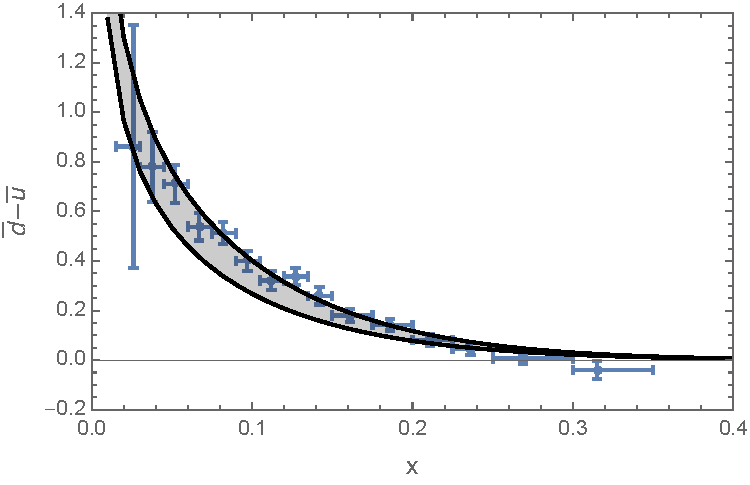
\includegraphics[width=0.6\linewidth]{rediff}
	\caption{The predicted $\bar{d}-\bar{u}$ from the meson cloud model and compared with the E866 results (blue symbol), taken from Ref.~\cite{alberg2022}.}
	\label{fig:pion_cloud}
\end{figure}

\subsection{Chiral Quark Model}
Similar to the meson cloud model, the chiral quark model~\cite{li1998} attributes the sea quarks to
the presence of Goldstone bosons in the nucleon. However, the Goldstone bosons in chiral quark model
are emitted from the valence quarks. The quark helicity would also be modified by the emission of a
spin-zero meson in P-wave, as indicated by the subscripts.
\begin{equation}
	q_{\pm} \rightarrow GB + q^\prime_\mp \rightarrow \left(q q^\prime\right)_0 q_{\mp}^\prime.
\end{equation}
For example, after one emission, the $u$ quark wavefunction would have the following components
\begin{equation}
	\Psi\left(u\right) \sim \left[d\pi^+ + s K^+ + u \left(\frac{\pi^0}{\sqrt{2}} + \frac{\eta}{\sqrt{6}}\right)\right],
\end{equation}
which can be expressed in terms of the quark contents by using $\pi^+ = u\bar{d}$ and $K^+ = u\bar{s}$. etc.
The probability of the transitions is given by squaring the wavefunction, and if
\begin{equation}
	Prob\left[ u_+ \rightarrow \pi^+d_-\right] \equiv a,
\end{equation}
and using charge asymmetry to determine the $d$ quark wavefunction, the number of antiquark after one emission
by the initial $(2u+d)$ valence quarks in the proton is given by
\begin{equation}
	\begin{aligned}
		\bar{u} \equiv \int^1_0 \dd{x}\bar{u}(x) & = 2\cross\frac{4}{9}a +a+\frac{1}{9}a = 2a,                         \\
		\bar{d} \equiv \int^1_0 \dd{x}\bar{d}(x) & = 2\cross\left(a+\frac{1}{9}a\right) + \frac{4}{9}a = \frac{8}{3}a.
	\end{aligned}
\end{equation}
Therefore the model predicts a light sea-quark asymmetry $\bar{d}-\bar{u} =\frac{2}{3}a $.
Unlike the meson cloud model, the Goldstone boson in the chiral quark model are emitted
by the valance quarks, which only carry a fraction of the total hadron's momentum.
Therefore the boson in the chiral quark model would necessarily carry a smaller momentum than
it would in the meson cloud model, and the sea-quark distributions would peak at a lower value of $x$ \cite{szczurek1996,peng1998}.



\subsection{Statistical Model}
In the statistical model~\cite{bourrely2015}, the nucleon is viewed as a gas of massless partons in equilibrium in
a finite volume. And the parton distributions at the initial scale would then be proportional to
\begin{equation}
	\left[ \exp\left[\left(x-X_{0p}\right)/\bar{x}\right] \pm 1 \right]^{-1},
\end{equation}
where the plus sign for the quarks and antiquarks corresponds to a Fermi-Dirac distribution and
the minus sign for gluons corresponds to a Bose-Einstein distribution. The constant $X_{0p}$
plays the role of the thermodynamic potential of the parton $p$ and $\bar{x}$ is the universal
temperature.

In this model, the potential of a quark $q_i^h$ with helicity $h$ has an opposite sign to that of the
potential of the corresponding antiquark $q_i^{-h}$ with helicity $-h$
\begin{equation}
	X_{0q}^h = -X_{0\bar{q}}^{-h}.
	\label{eq:stat_potential}
\end{equation}
Since there are more $u$ quarks than $d$ quarks in the proton, one would expect
\begin{equation}
	X_{0u}^+ + X_{0u}^- > X_{0d}^+ + X_{0d}^-,
\end{equation}
and combining with \cref{eq:stat_potential}, one would expect $\bar{d} > \bar{u}$ in the proton.
And this is shown in \cref{fig:stat_dbub}.
\begin{figure}[h]
	\centering
	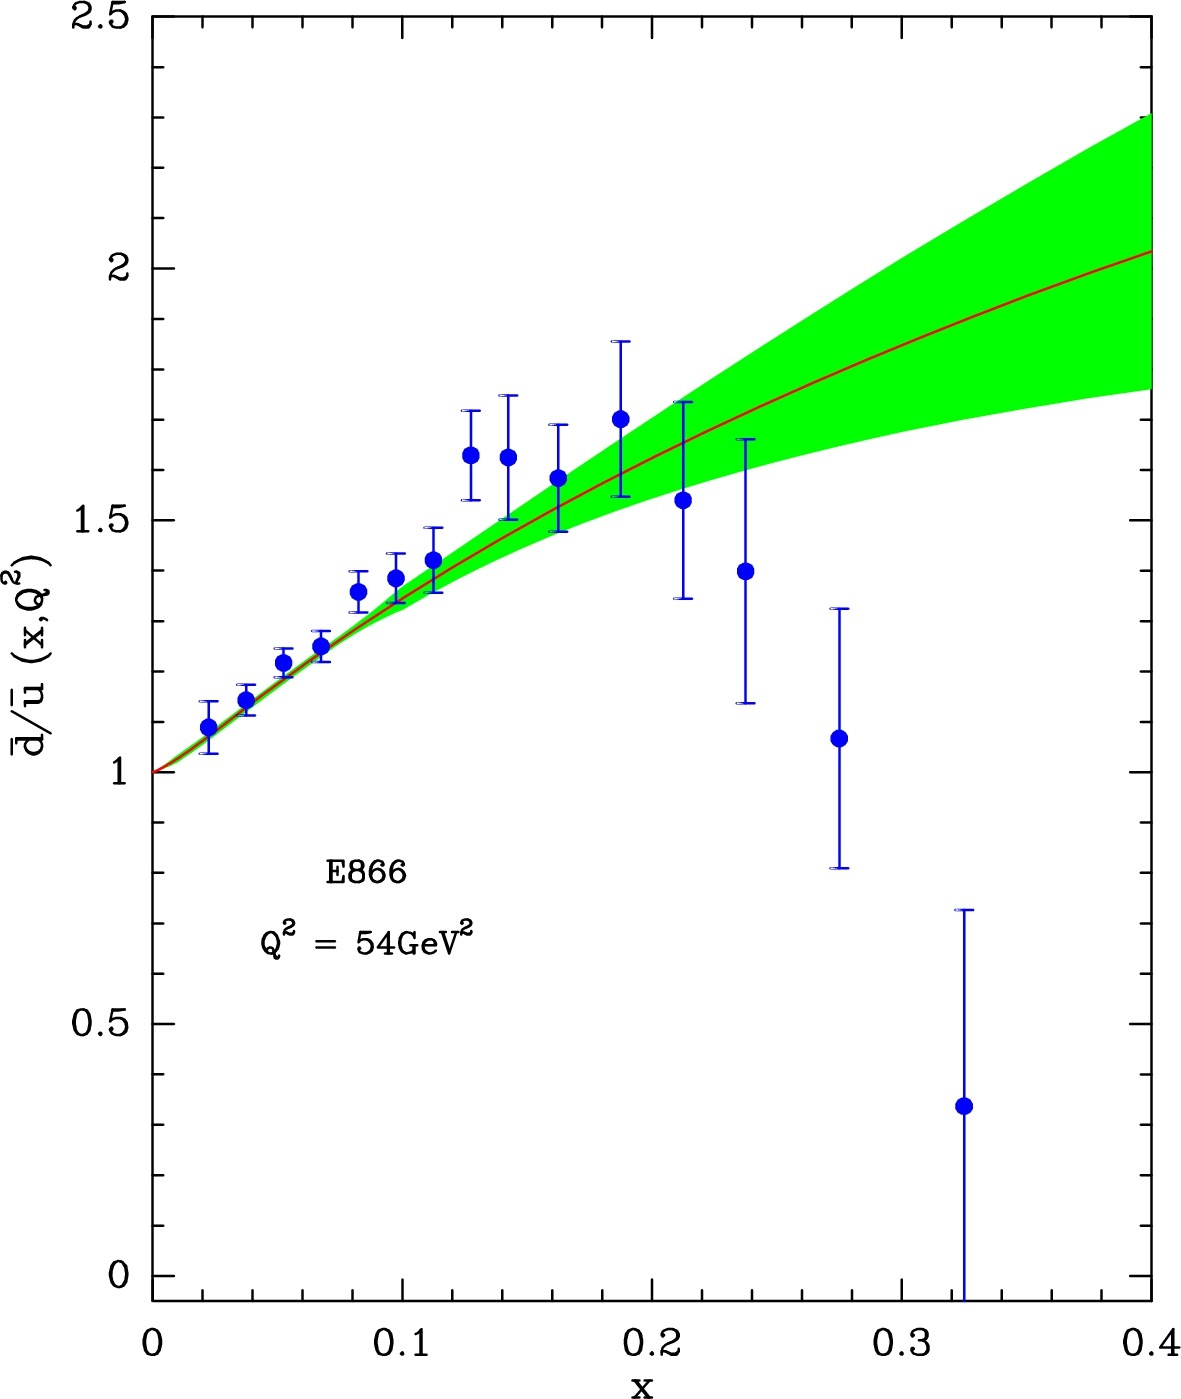
\includegraphics[width=0.5\linewidth]{statistical_model}
	\caption{The extracted light sea-quark asymmetry from the statistical model and compared with E866, taken
		from Ref.~\cite{soffer2019}.}
	\label{fig:stat_dbub}
\end{figure}


\subsection{Five-quark Intrinsic Sea Model}
In the 1980s, Brodsky, Hoyer, Peterson and Sakai (BHPS)~\cite{brodsky1980} proposed
the possible existence of a significant $\ket{uudc\bar{c}}$ five-quark Fock state component
in the proton in order to explain the larger than expected charmed hadrons production rate.

For a $\ket{uudQ\bar{Q}}$ proton Fock state, the probability for quark $i$ to carry a momentum
fraction $x_i$ is given by
\begin{equation}
	P\left(x_1,\cdots,x_2\right)=N_5 \delta\left(1-\sum^5_{i=1}x_i\right)\left[m_p^2-\sum^5_{i=1}\frac{m_i^2}{x_i}\right]^{-2},
\end{equation}
where the delta function ensures momentum conservation. $N_5$ is the normalization factor,
and $m_i$ is the mass of quark $i$.

Since the BHPS model also predicts the probability for the $\ket{uudQ\bar{Q}}$ configuration to
be proportional to $1/m^2_Q$, where $m_Q$ is the mass of quark $Q$, the intrinsic sea can have important
contribution to the light sea-quarks. In Refs.~\cite{chang2011,chang2011a}, the BHPS model
was extended to the light quark sector. In this model, the $\bar{u}$ and $\bar{d}$ are predicted
to  have the same $x$ dependence if one assumes $m_u=m_d$. The only source of asymmetry
are the probabilities of the $\ket{uudd\bar{d}}$ and $\ket{uudu\bar{u}}$ configurations,
which are not known from the BHPS model, and remain to be determined from experiments.
Nevertheless, the $x$ dependence of the $\bar{d}-\bar{u}$ asymmetry can be obtained from the model.
\Cref{fig:five_quark} shows the comparison of the $\bar{d}-\bar{u}$ data from E866 with calculation
based on BHPS model, with normalization fixed by the measured asymmetry. At the initial scale,
the sea-quark distribution exhibit a valence like behavior. As the scale increases, the distribution
becomes softer.
\begin{figure}[hb!]
	\centering
	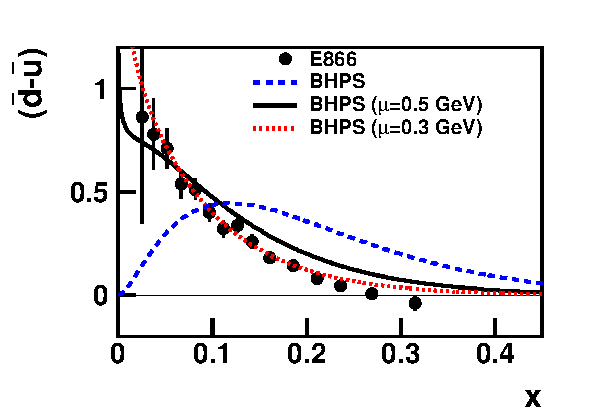
\includegraphics[width=0.6\linewidth]{fig_dbarubar}
	\caption{Comparison of the $\bar{d}-\bar{u}$ data with calculation based on BHPS model.
		The dashed curve corresponds the distribution at initial scale, and the solid and dotted
		curve are obtained by evolving to $Q^2=\SI{54}{\GeV\squared}$ assuming different initial scale $\mu$.
		Taken from Ref.~\cite{chang2011}. }
	\label{fig:five_quark}
\end{figure}

Recent global analysis from NNPDF~\cite{ball2022} and measurement from the LHCb~\cite{aaij2022}
have suggested evidence of intrinsic charm in the proton. This has led to many recent theory
development in understanding the non-perturbative charm in the proton~\cite{guzzi2023}. There are
also suggestions that SeaQuest kinematic would be ideal for testing limits on intrinsic charm~\cite{vogt2021}.

\subsection{Lattice QCD}
\label{subsec:lattice}
Lattice QCD calculations of the $\bar{d} - \bar{u}$ based on the Large Momentum Effective
theory (LaMET)~\cite{ji2021,constantinou2021} have become available recently by two different groups,
LP3~\cite{chen2018} and ETMC~\cite{alexandrou2018}.
The parton distribution functions described quarks and gluons in hadrons traveling at infinite
momentum. The principle for LaMET comes from the observation that the structure of the proton is
approximately independent of its momentum so long as it is much larger than the strong interaction
scale or its mass. Therefore the partonic structure can be calculated for a proton with
moderately-large momentum and taking the limit of the proton momentum to infinity.

\begin{figure}[h!]
	\centering
	\begin{subfigure}{0.45\linewidth}
		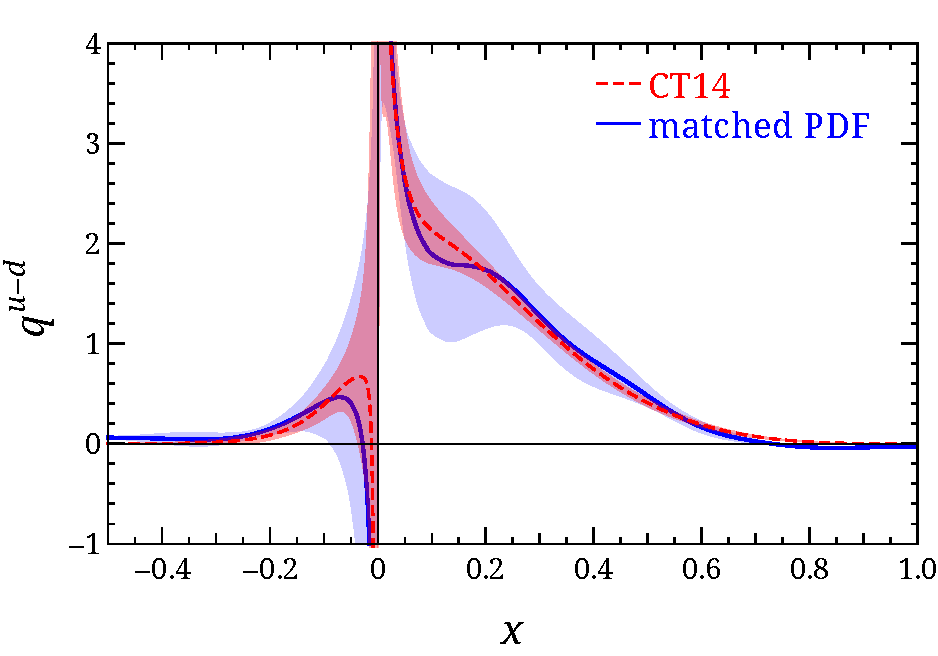
\includegraphics[width=\linewidth]{LP3-PDF-CT14}
	\end{subfigure}
	\begin{subfigure}{0.45\linewidth}
		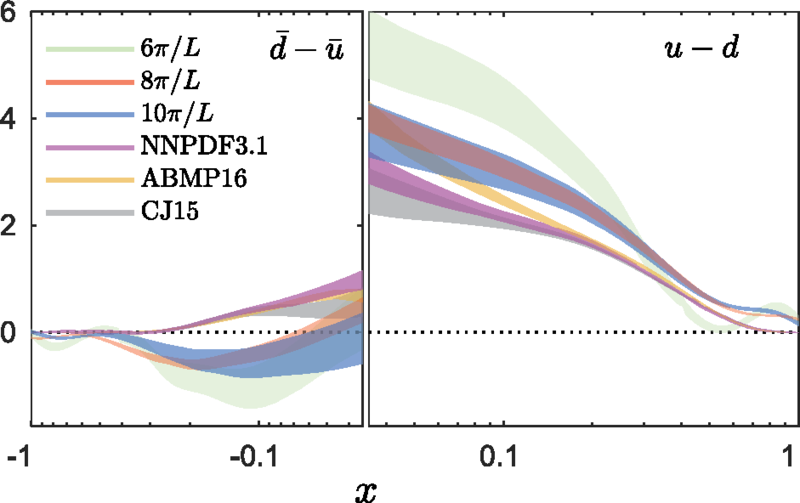
\includegraphics[width=\linewidth]{alexandrou2018}
	\end{subfigure}
	\caption{The calculated isovector PDF from the LP3 collaboration (left)~\cite{chen2018}
		and ETMC (right)~\cite{alexandrou2018}.
		The negative $x$ region denote $\bar{d}-\bar{u}$ at $\left|x\right|$.}
	\label{fig:lamet}
\end{figure}
LaMET are typically used to calculate flavor non-singlet quantities such as $u-d$ and $\bar{d}-\bar{u}$,
as the disconnected diagram would cancel out in the calculation.
\Cref{fig:lamet} shows the results using LaMET from two different groups and are compared with
different global PDF extractions. While the result by the LP3 collaboration
is in good agreement with CT14, the result from the ETMC group differs from the PDFs,
especially in the antiquark region.

\chapter{Charmonium Production}
\label{ch:jpsi}
Another process for probing the nucleon structure is the charmonium production~\cite{peng1995,chang2020}.
Unlike DIS and Drell-Yan, the charmonium production involves strong interaction already
at the leading-order. Therefore it can be used to probe the gluon structure, which 
the DIS or Drell-Yan processes are less sensitive to, and the quark and anti-quark structures.
At leading order, charmonium production involves two sub-processes, gluon fusion and
quark-antiquark annihilation into a gluon, as illustrated in \cref{fig:charmonium}.

The simultaneous measurement of charmonium production and Drell-Yan process, two very different
processes, can provide complementary information on the partonic structures of the nucleon.
In particular, the $\sigma_{pd}/2\sigma_{pp}$ ratio for charmonium
production is expected to be sensitive to the ratio of the gluon distributions in the proton
and neutron, as well as the $\bar{d}/\bar{u}$ ratio in the proton.

If quark-antiquark annihilation is the dominant process for charmonium
production, the $\sigma_{pd}/2\sigma_{pp}$ ratio would provide an
independent measurement of the $\bar{d}/ \bar{u}$ flavor asymmetry in the
proton~\cite{peng1995}, complementary to the Drell-Yan process.
On the other hand, if gluon-gluon fusion is the dominant process, the
$\sigma_{pd}/2\sigma_{pp}$ ratio could probe the relative gluon content
in the proton and neutron, providing a test of the charge symmetry at the partonic level.
Violation of charge symmetry is predicted at both the hadronic~\cite{stephenson2003,opper2003}
and the partonic levels~\cite{londergan2010}. Since gluon is an iso-scalar particle,
charge symmetry requires that the gluon distributions in the proton and neutron
are identical. A measurement of the gluon contents in proton and neutron could test charge symmetry at
the partonic level~\cite{piller1996,zhu2008,lansberg2012}.

As $J/\psi$ and $\psi'$ are resonances, they show up as peaks in the dimuon mass spectrum,
and the cross section is significantly larger than the Drell-Yan cross section.
However, there are various models for calculating the quarkonium production,
which contains non-perturbative aspects of QCD.
The models usually separate the production
mechanism into two parts, the production of heavy-quark pairs and their subsequent
hadronization into quarkonium states. One of the early approaches is the Color
Evaporation Model (CEM)~\cite{einhorn1975,bodwin1995}. The heavy-quark
pairs production is expanded in terms of the strong coupling constant $\alpha_s$
and is calculated with perturbative QCD (pQCD). CEM then assumes a constant
probability $F$ for the $c\bar{c}$ pairs to hadronize into a specific quarkonium
state and this probability is independent of the kinematics or the production
sub-process. The $J/\psi$ production cross section in the CEM framework can be
expressed as
\begin{equation}
	\begin{split}
		\left.\frac{d\sigma}{dx_F}\right|_{J/\psi} & = F \sum_{i,j = q,\bar{q},G}\int^{2m_D}_{2m_c} dM_{c\bar{c}}  \frac{2M_{c\bar{c}}}{s\sqrt{x_F^2+4M_{c\bar{c}}^2/s}}                                 \\
		                                           & \cross f_{i/A}\left(x_1,\mu_F\right)f_{j/B}\left(x_2,\mu_F\right)\sigma\left[ij\rightarrow c\bar{c}X\right]\left(x_1P_A,x_2P_B,\mu_F,\mu_R \right),
	\end{split}
\end{equation}
where $i$, $j$ denote the type of interacting partons.
\begin{figure}[htpb!]
	\centering
	\begin{subfigure}[c]{0.4\linewidth}
		\begin{subfigure}[c]{\linewidth}
			\begin{tikzpicture}
	\tikzstyle{every node}=[font=\large]
	\begin{feynman}
		\vertex  (a1);
		\vertex [right= of a1, blob] (a2) {};
		\vertex [right= 2cm of a2] (a3) ;
		\vertex [below= 3cm of a1] (b1);
		\vertex [below= 3cm of a2,blob] (b2) {};
		\vertex[below= 3cm of a3] (b3);
		\vertex  at ($(b2) + (1cm , +1.5cm)$) [dot] (d);
		\vertex [right= 2cm of d] (d1);
		\vertex at ($(d1) + (1cm , +1.2cm)$) (c1) {$c$};
		\vertex at ($(d1) + (1cm , -1.2cm)$) (c2) {$\bar{c}$};
		\diagram*{
		(a1) --[fermion](a2),
		(a2) --[double distance=4pt, thick](a3),
		(b1) --[fermion](b2),
		(b2) --[double distance=4pt, thick](b3),
		(b2) --[gluon, edge label'=$g$] (d),
		(a2) --[gluon, edge label=$g$](d),
		(d) --[gluon](d1),
		(c2) --[fermion] (d1);
		(d1) --[fermion] (c1);
		};
	\end{feynman}
\end{tikzpicture}

		\end{subfigure}
		\begin{subfigure}[c]{\linewidth}
			\begin{tikzpicture}
	\tikzstyle{every node}=[font=\large]
	\begin{feynman}
		\vertex  (a1);
		\vertex [right= of a1, blob] (a2) {};
		\vertex [right= 2cm of a2] (a3) ;
		\vertex [below= 3cm of a1] (b1);
		\vertex [below= 3cm of a2,blob] (b2) {};
		\vertex [below= 3cm of a3] (b3);
		\vertex  at ($(b2) + (1.5cm , +1cm)$) [dot] (d);
		\vertex [above= 1cm of d] (d1);
		\vertex [right= 2.25cm of d1] (c1) {$c$};
		\vertex [right= 2.25cm of d] (c2) {$\bar{c}$};
		\diagram*{
		(a1) --[fermion](a2),
		(a2) --[double distance=4pt, thick](a3),
		(b1) --[fermion](b2),
		(b2) --[double distance=4pt, thick](b3),
		(b2) --[gluon, edge label=$g$] (d),

		(a2) --[gluon, edge label'=$g$](d1),
		(d) --[fermion](d1),
		(d1) --[fermion] (c1);
		(c2) --[fermion] (d);
		};
	\end{feynman}
\end{tikzpicture}

		\end{subfigure}
		\caption{Gluon fusion\label{subfig:gluon}.}
	\end{subfigure}
	\quad
	\begin{subfigure}[c]{0.4\linewidth}
		\begin{tikzpicture}
	\tikzstyle{every node}=[font=\large]
	\begin{feynman}
		\vertex  (a1);
		\vertex [right= of a1, blob] (a2) {};
		\vertex [right= 2cm of a2] (a3) ;
		\vertex [below= 3cm of a1] (b1);
		\vertex [below= 3cm of a2,blob] (b2) {};
		\vertex[below= 3cm of a3] (b3);
		\vertex  at ($(b2) + (1cm , +1.5cm)$) [dot] (d);
		\vertex [right= 2cm of d] (d1);
		\vertex at ($(d1) + (1cm , +1.2cm)$) (c1) {$c$};
		\vertex at ($(d1) + (1cm , -1.2cm)$) (c2) {$\bar{c}$};
		\diagram*{
		(a1) --[fermion](a2),
		(a2) --[double distance=4pt, thick](a3),
		(b1) --[fermion](b2),
		(b2) --[double distance=4pt, thick](b3),
		(b2) --[anti fermion, edge label'=$\bar{q}$] (d),
		(a2) --[fermion, edge label=$q$](d),
		(d) --[gluon](d1),
		(c2) --[fermion] (d1);
		(d1) --[fermion] (c1);
		};
	\end{feynman}
\end{tikzpicture}

		\caption{Quark-antiquark annihilation.\label{subfig:qqbar}}
	\end{subfigure}
	\caption{The Feynman diagrams for $c\bar{c}$ pair production.}
	\label{fig:charmonium}
\end{figure}
While proton induced $J/\psi$ production is often dominated by gluon fusion
process~\cite{vogt1999}, the relative importance of gluon fusion
and quark-antiquark annihilation is a strong function of hadron-hadron center-of-mass energy $\sqrt{s}$
and $x_F=2P_L/\sqrt{s}$, where $P_L$ is the longitudinal momentum of the $J/\psi$ meson in the
hadron-hadron center-of-mass frame.
The NA51 collaboration reported a measurement of the $p+p$ and $p+d$ cross sections
for the charmonium at \SI{450}{\GeV} at a single value of rapidity ($x_F\sim 0$)~\cite{abreu1998}.
The SeaQuest measurement covers a broader kinematic range of $0.5<x_F<0.9$ at a lower beam energy
of \SI{120}{\GeV}.
The calculated cross section for $J/\psi$ production in $p+p$ at \SI{120}{\GeV} using
CEM is shown in \cref{fig:cem_cs}.
At our beam energy, the quark-antiquark annihilation would be more important than gluon fusion at large $x_F$, where
the SeaQuest experiment has better coverage.
\begin{figure}[h!]
	\centering
	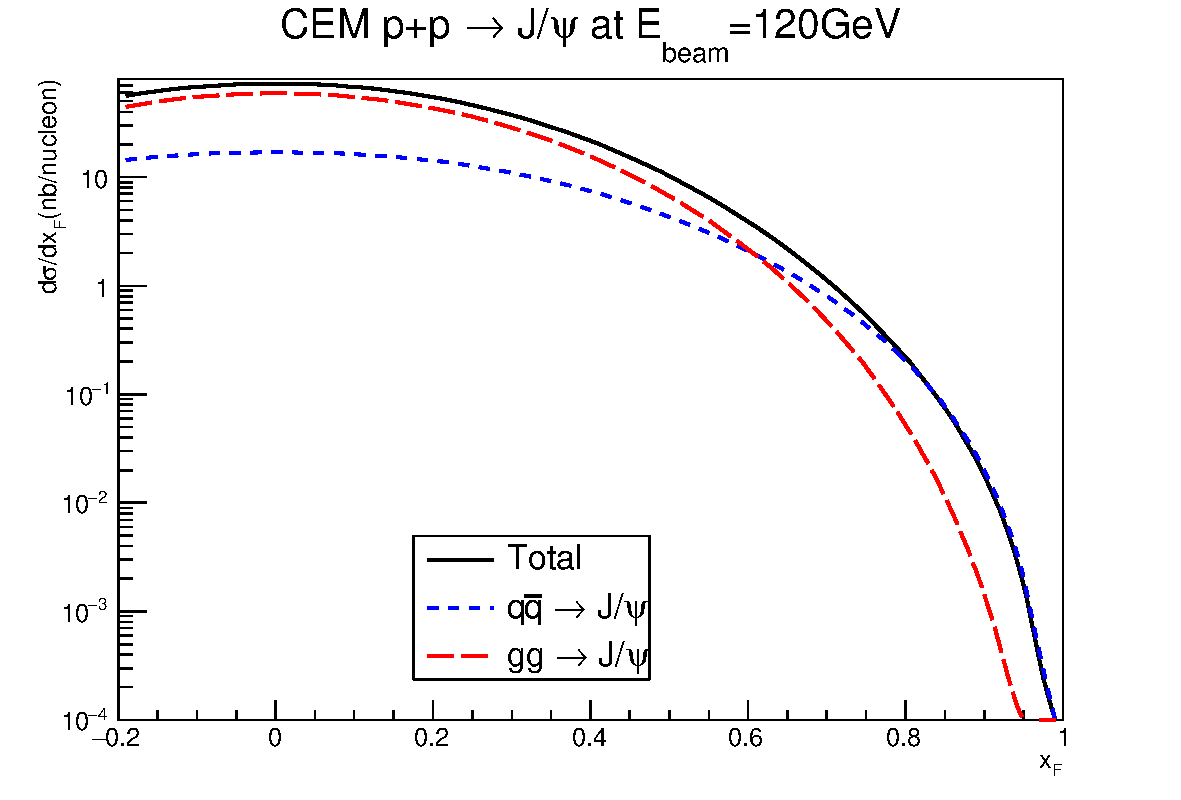
\includegraphics[width=0.45\linewidth]{pp_norm_cs_NLO_pp}
	\caption{Calculated cross section for $J/\psi$ production using the CEM model with the CT14NLO PDF.
		The CEM code is obtained from Ref.~\cite{mangano1993}.}
	\label{fig:cem_cs}
\end{figure}

Another theoretical model for quarkonium production is the non-relativistic
QCD (NRQCD) \cite{bodwin1995}. Unlike CEM, the probability of
hadronization depends on the color and spin state of the $c\bar{c}$ pairs and
is described by various long-distance matrix elements (LDMEs). The quarkonium
production cross section in this framework is given as
\begin{equation}
	\begin{split}
		\frac{d\sigma^H}{dx_F} & =\sum_{i,j = q,\bar{q},G}\int^1_0 dx_1 dx_2 \delta(x_F-x_1+x_2)                                                                                        \\
		                       & \cross f_{i/A}\left(x_1,\mu_F\right)f_{j/B}\left(x_2,\mu_F\right)\hat{\sigma}\left[ij\rightarrow H\right]\left(x_1P_A,x_2P_B,\mu_F,\mu_R , m_c\right),
	\end{split}
\end{equation}
\begin{equation}
	\hat{\sigma}\left[ij\rightarrow H\right]= \sum_n C^{ij}_{c\bar{c}\left[n\right]}\left(x_1P_A,x_2P_B,\mu_F,\mu_R , m_c\right)\expval{O^H_n}.
\end{equation}
The $c\bar{c}$ pairs are produced in state $n={^{2S+1}L_J^{\left[a\right]}}$ with definite spin $S$,
orbital angular momentum $L$, total angular momentum $J$, and color state $a=1,8$.
The coefficient $C^{ij}_{c\bar{c}\left[n\right]}$ describes the production of $c\bar{c}$ pair in state $n$,
from partons $i$ and $j$ and is calculated perturbatively in powers of $\alpha_s$ using pQCD.
The LDME $\expval{O^H_n}$ accounts for the hadronization probability for a specific $c\bar{c}$ state $n$ into the
charmonium state $H$.
This formalism suggests that the $c\bar{c}$ pairs can be produced in color-octet state,
then evolve into physical color-singlet quarkonia by non-perturbative emission of soft gluons.

The LDMEs describe the hadronization process,
and are assumed to be universal and independent of beam or target hadrons and the energy scale.
As the LDMEs describe the non-perturbative interactions,
they cannot be calculated using pQCD, and have to be extracted from models or experiments.
For example, the color-singlet LDMEs are typically estimated using the potential model~\cite{eichten1995}.
Using the potential model, the wavefunction of the heavy quark pair can be calculated, 
and the color-singlet LDMEs can be estimated from the wavefunction at the origin
\begin{equation}
	\begin{split}
		\expval{O^{\psi}\left[^3S_1^{\left[1\right]}\right]} &= \frac{3N_c}{2\pi} \left| R_{\psi}\left(0\right)\right|^2,\\
		\expval{O^{\chi_{cJ}}\left[^3P_J^{\left[1\right]}\right]} &= \frac{3}{4\pi}\left(2J+1\right) \left| R'_{\chi_{cJ}}\left(0\right)\right|^2.
	\end{split}
\end{equation}
And the potential model gives $\left|R_{J/\psi}\left(0\right)\right|^2=\SI{0.81}{\GeV^3}$,
$\left|R_{\psi'}\left(0\right)\right|^2=\SI{0.53}{\GeV^3}$, and $\left|R'_{\chi_{cJ}}\left(0\right)\right|^2=\SI{0.075}{\GeV^5}$.
The other LDMEs are typically obtained by fitting to data.
Some existing LDMEs for direct $J/\psi$ and $\psi'$ productions are tabulated in \cref{tab:LDMEs}.
The values of some LDMEs from different groups are very different, in some cases, even the signs are different.
This is partly due to the choice of data sets used in their global fits. The
SeaQuest experiment can provide additional constraints on these LDMEs. Some
existing data are shown in \cref{fig:charm_cs}.
Unlike most previous fixed-target charmonium experiments, which utilized nuclear
targets, SeaQuest have both hydrogen and deuterium targets.
Studying the charmonium production in $p+p$ and $p+d$ would allow the extraction
of the LDMEs with little, if any, model dependence from nuclear effects.

\begin{table}[ht!]
	\centering
	\caption{The NRQCD LDMEs for $J/\psi$ and $\psi'$ from different groups.}
	\label{tab:LDMEs}
	\begin{adjustbox}{width=1.03\textwidth, center=\textwidth}
		\begin{tabular}{c|ccccc}
	\hline
	                                                            & Bodwin et al~\cite{bodwin2016} & Butenschoen et al~\cite{butenschoen2011,butenschoen2023} & Chao et al~\cite{chao2012} & Gong et al~\cite{gong2013} & Feng et al~\cite{feng2019} \\ \hline
	$\expval{ O^{J/\psi}[^3S_1^{\left[1\right]}]}$ (\unit{\GeV^3})        & \num{1.32}                     & \num{1.32}                                               & \num{1.16}                 & \num{1.16}                 & \num{1.16}                 \\ \hline
	$\expval{ O^{J/\psi}[^1S_0^{\left[8\right]}]}$ (\unit{10^{-2}\GeV^3}) & \num{-0.713\pm0.364}           & \num{3.04\pm0.35}                                        & \num{8.9\pm0.98}           & \num{9.7\pm0.9}            & \num{5.66\pm0.47}          \\ \hline
	$\expval{ O^{J/\psi}[^3S_1^{\left[8\right]}]}$ (\unit{10^{-2}\GeV^3}) & \num{11.0\pm1.4}               & \num{0.168\pm0.046}                                      & \num{0.30\pm0.12}          & \num{-0.46\pm0.13}         & \num{0.177\pm0.058}        \\ \hline
	$\expval{ O^{J/\psi}[^3P_0^{\left[8\right]}]}$ (\unit{10^{-2}\GeV^5}) & \num{0.702\pm0.340}            & \num{-0.908\pm0.161}                                     & \num{1.26\pm0.50}          & \num{-2.14\pm0.56}         & \num{0.770\pm0.230}        \\ \hline \hline
	$\expval{ O^{\psi'}[^3S_1^{\left[1\right]}]}$ (\unit{\GeV^3})         & \num{0.76}                     & \num{0.76}                                               & ---                        & \num{0.758}                & ---                        \\ \hline
	$\expval{ O^{\psi'}[^1S_0^{\left[8\right]}]}$ (\unit{10^{-2}\GeV^3})  & \num{-0.157\pm0.280}           & \num{0.0958\pm0.0129}                                    & ---                        & \num{-0.012\pm0.869}       & ---                        \\ \hline
	$\expval{ O^{\psi'}[^3S_1^{\left[8\right]}]}$ (\unit{10^{-2}\GeV^3})  & \num{3.14\pm0.79}              & \num{0.149\pm0.001}                                      & ---                        & \num{0.34\pm0.12}          & ---                        \\ \hline
	$\expval{ O^{\psi'}[^3P_0^{\left[8\right]}]}$ (\unit{10^{-2}\GeV^5})  & \num{-0.257\pm0.272}           & \num{-0.0583\pm0.0056}                                   & ---                        & \num{0.945\pm0.54}         & ---                        \\ \hline
\end{tabular}
	\end{adjustbox}
\end{table}

\begin{figure}[ht!]
	\centering
	\begin{subfigure}{0.48\linewidth}
		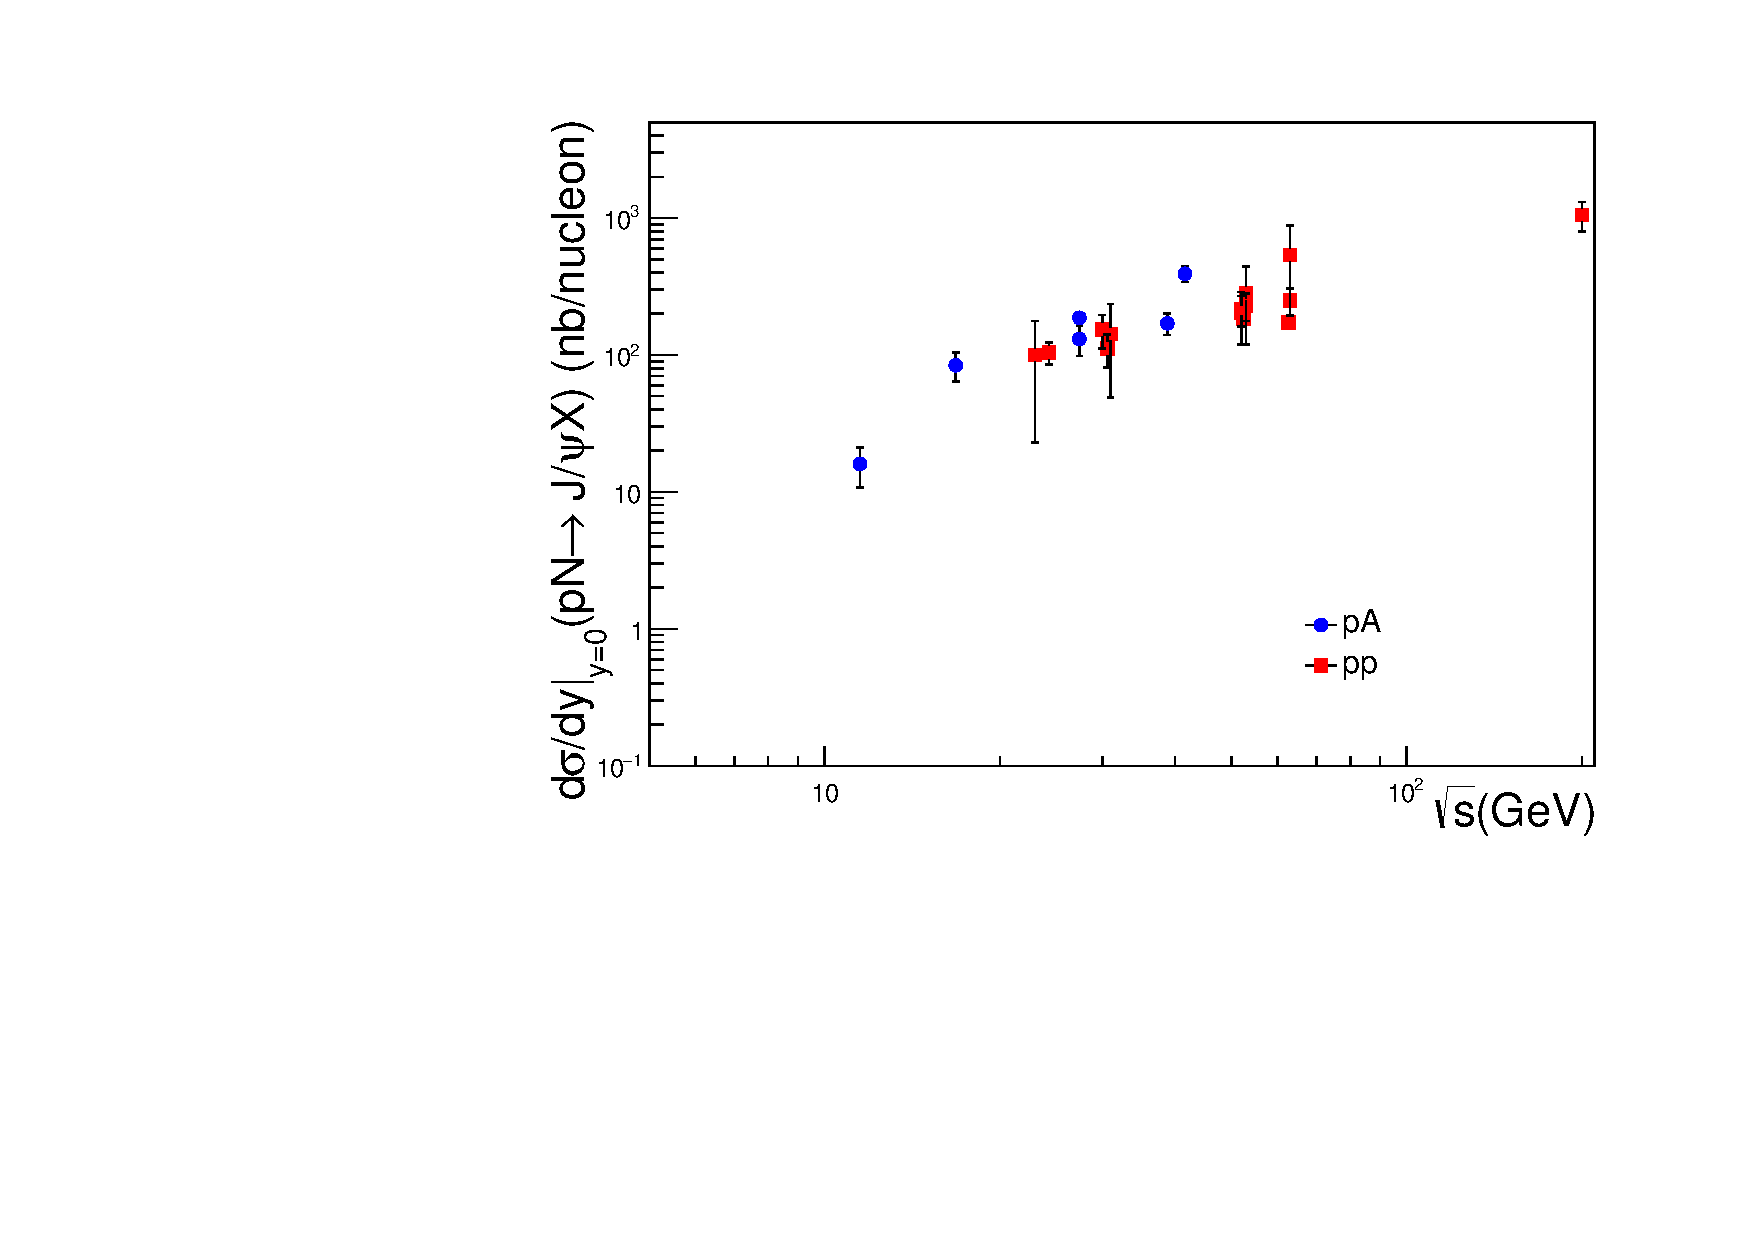
\includegraphics[width=\linewidth]{cs/sigma0}
	\end{subfigure}
	\begin{subfigure}{0.48\linewidth}
		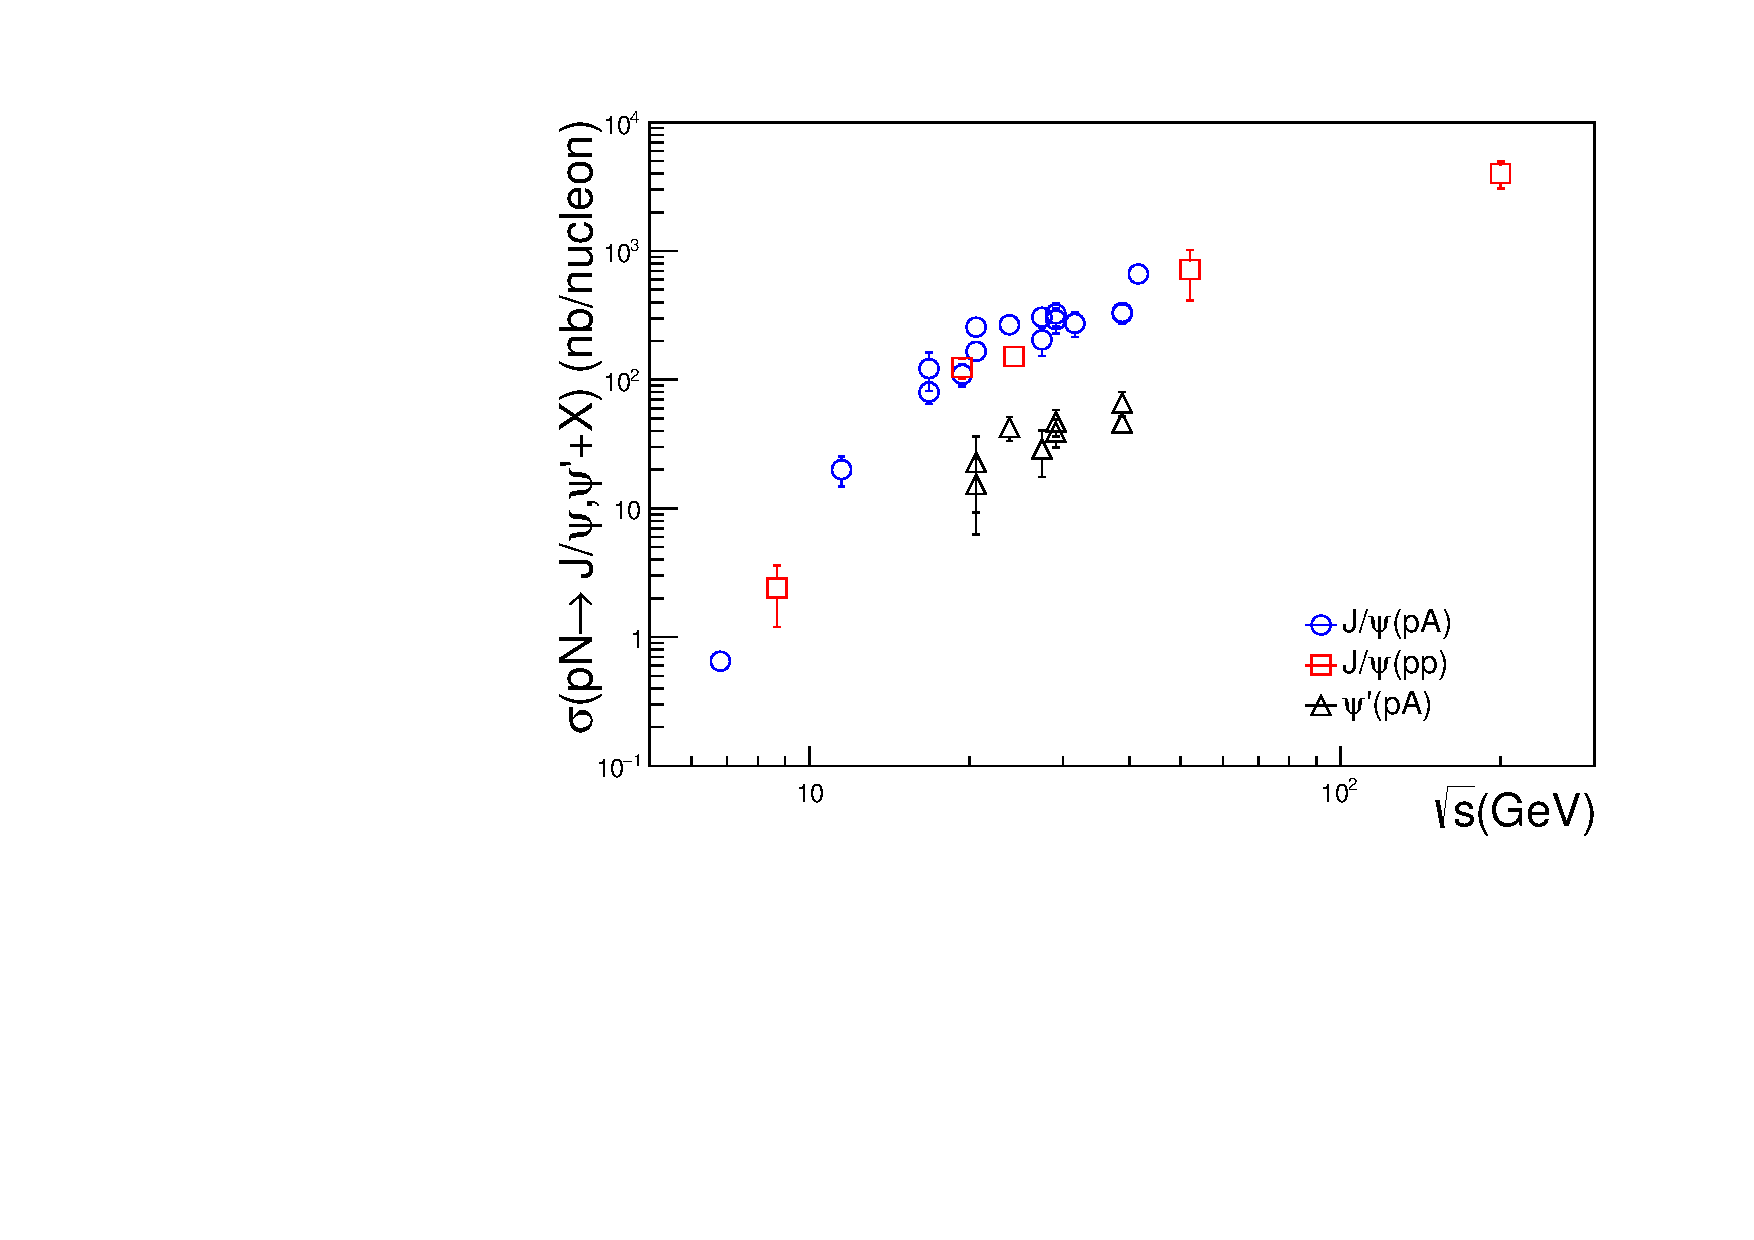
\includegraphics[width=\linewidth]{cs/sigmaTotal}
	\end{subfigure}
	\caption{The differential production cross sections at $y=0$ (left) and total
		cross section (right) in proton-proton ($pp$) and proton-nucleus ($pA$) interactions
		as a function of $\sqrt{s}$, adapted from Ref.~\cite{maltoni2006}.}
	\label{fig:charm_cs}
\end{figure}

The NRQCD calculations~\cite{chang2023a} presented in this thesis are performed using the LDMEs
from a recent global analysis of both pion- and proton-induced charmonium production data~\cite{chang2023}.
In the their analysis, only unpolarized observables were analyzed.
Therefore, the formalism can be simplified by combining the color-octet LDMEs
\begin{equation}
	\Delta^H_{[8]}=\expval{O^H\left[^1S_0^{\left[8\right]}\right]}+\frac{3}{m_c^2}\expval{O^H\left[^3P_0^{\left[8\right]}\right]}+\frac{4}{5m_c^2}\expval{O^H\left[^3P_2^{\left[8\right]}\right]}.
\end{equation}
Furthermore, the calculated cross section for $J/\psi$ also need to include the feed-down from hadronic decay
of $\psi'$ and radiative decays of three $\chi_{cJ}$ states.
Therefore the total $J/\psi$ cross section is given by
\begin{equation}
	\sigma_{J/\psi}=\sigma_{J/\psi}^{\mathrm{direct}}+B\left(\psi'\to J/\psi X\right)\sigma_{\psi'} +\sum_{J=0}^2 B\left(\chi_{cJ}\to J/\psi\gamma\right) \sigma_{\chi_{cJ}},
\end{equation}
where $B$ is the branching ratio for $\psi'$ or $\chi_{cJ}$ to decay into $J/\psi$.

The relationship between the LDMEs and the $c\bar{c}$ produced via different
sub-processes up to $\mathcal{O}\left(\alpha_s^3\right)$ are shown in \cref{tab:LDME_order}.
For $q\bar{q}$ sub-process, the $c\bar{c}$ pairs are produced in
$S$-wave color-octet states at $\mathcal{O}\left(\alpha_s^2\right)$,
which then hadronize into various charmonium states with the LDMEs $\expval{O^H\left[^3 S_1^{[8]}\right]}$.
The $J/\psi$ and $\psi'$ mesons can also be produced via $GG$ sub-process.
The $c\bar{c}$ pairs produced are either in color-singlet
state at $\mathcal{O}\left(\alpha_s^3\right)$ or color-octet state at $\mathcal{O}\left(\alpha_s^2\right)$.

The number of independent LDMEs are further reduced by applying spin symmetry relations
\begin{equation}
	\begin{split}
		\expval{O^{J/\psi,\psi'}\left[^3P_j^{\left[8\right]}\right]} & = \left(2J+1\right)\expval{O^{J/\psi,\psi'}\left[^3P_0^{\left[8\right]}\right]} \quad \text{for }J=2 \\
		\expval{O^{\chi_{cJ}}\left[^3S_1^{\left[8\right]}\right]}    & = \left(2J+1\right)\expval{O^{\chi_{c0}}\left[^3S_1^{\left[8\right]}\right]} \quad \text{for }J=1,2  \\
		\expval{O^{\chi_{cJ}}\left[^3P_J^{\left[1\right]}\right]}    & = \left(2J+1\right)\expval{O^{\chi_{c0}}\left[^3P_0^{\left[1\right]}\right]} \quad \text{for }J=1,2.
	\end{split}
\end{equation}
\begin{table}[h!]
	\centering
	\caption{Relationship of the LDMEs and the associated order of $\alpha_s$ to
		the scattering sub-processes for various charmonium states.}
	\label{tab:LDME_order}
	{
\renewcommand{\arraystretch}{1.5}
\begin{tabular}{cccc}
	\hline
	$H$                                                                                                                                                                            &
	$q\bar{q}$                                                                                                                                                                     &
	$GG$                                                                                                                                                                           &
	$qG$                                                                                                                                                                             \\ \hline
	$J/\psi,\,\psi'$                                                                                                                                                               &
	$\expval{ O^H\left[^3S_1^{\left[8\right]}\right]}\, \left(\alpha_s^2\right)$                                                                                                   &
	\begin{tabular}[c]{@{}c@{}}$\Delta_{[8]}^H \, \left(\alpha^2_s\right)$\\ $\expval{ O^H\left[^3S_1^{\left[1\right]}\right]}\, \left(\alpha_s^3\right)$\end{tabular} &
	\\
	$\chi_{c0}$                                                                                                                                                                    &
	$\expval{ O^H\left[^3S_1^{\left[8\right]}\right]}\, \left(\alpha_s^2\right)$                                                                                                   &
	$\expval{ O^H\left[^3P_0^{\left[1\right]}\right]}\, \left(\alpha_s^2\right)$                                                                                                   &
	\\
	$\chi_{c1}$                                                                                                                                                                    &
	$\expval{ O^H\left[^3S_1^{\left[8\right]}\right]}\, \left(\alpha_s^2\right)$                                                                                                   &
	$\expval{ O^H\left[^3P_1^{\left[1\right]}\right]}\, \left(\alpha_s^3\right)$                                                                                                   &
	$\expval{ O^H\left[^3P_1^{\left[1\right]}\right]}\, \left(\alpha_s^3\right)$                                                                                                     \\
	$\chi_{c2}$                                                                                                                                                                    &
	$\expval{ O^H\left[^3S_1^{\left[8\right]}\right]}\, \left(\alpha_s^2\right)$                                                                                                   &
	$\expval{ O^H\left[^3P_2^{\left[1\right]}\right]}\, \left(\alpha_s^2\right)$                                                                                                   &
	\\ \hline
\end{tabular}
}
\end{table}
\begin{table}[h!]
	\centering
	\caption{The values of LDMEs used in the NRQCD calculations shown in this thesis,
		taken from Ref.~\cite{chang2023}.}
	\label{tab:LDME_wcchang}
	\begin{tabular}{ccccc}
\hline
$H$ &
  $\expval{O^H\left[^3S_1^{\left[1\right]}\right]}$ &
  $\expval{O^H\left[^3S_1^{\left[8\right]}\right]}$ &
  $\Delta_{[8]}^H$ &
  $\expval{O^H\left[^3P_0^{\left[1\right]}\right]}$ \\ \hline
$J/\psi$    & $1.16$ & $0.0259\pm 0.0023$ & $0.0560\pm0.0016$ &         \\
$\psi'$     & $0.76$ & $0.0132\pm 0.0009$ & $0.0057\pm0.0003$ &         \\
$\chi_{cJ}$ &        & $0.0032$           &                   & $0.044$ \\ \hline
\end{tabular}

\end{table}

The values of LDMEs used in the calculations are tabulated in \cref{tab:LDME_wcchang}.
The calculated cross sections for $J/\psi$ and $\psi'$ production using NRQCD for
$p+p$ at 120 GeV are shown in \cref{fig:NRQCD_cs}. In this model, quark-antiquark
annihilation is more important than suggested by CEM. This model also suggests
that the relative importance of the two sub-processes depend on the charmonium state.
In particular, \cref{fig:NRQCD_cs} shows that the quark-antiquark annihilation
is the dominant process for $\psi^\prime$ production.
\begin{figure}[h!]
	\centering
	\begin{subfigure}{0.45\linewidth}
		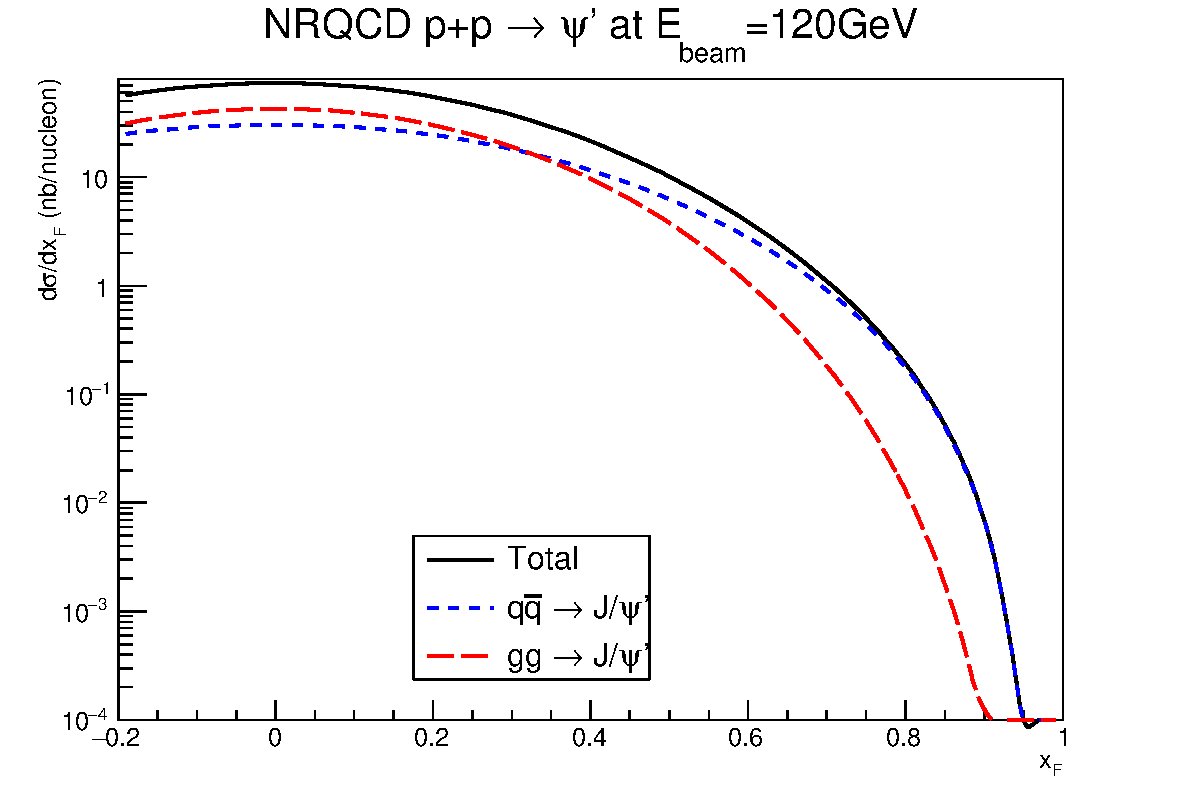
\includegraphics[width=\linewidth]{jpsi_cs_pp}
		\caption{$J/\psi$ production.}
	\end{subfigure}
	\quad
	\begin{subfigure}{0.45\linewidth}
		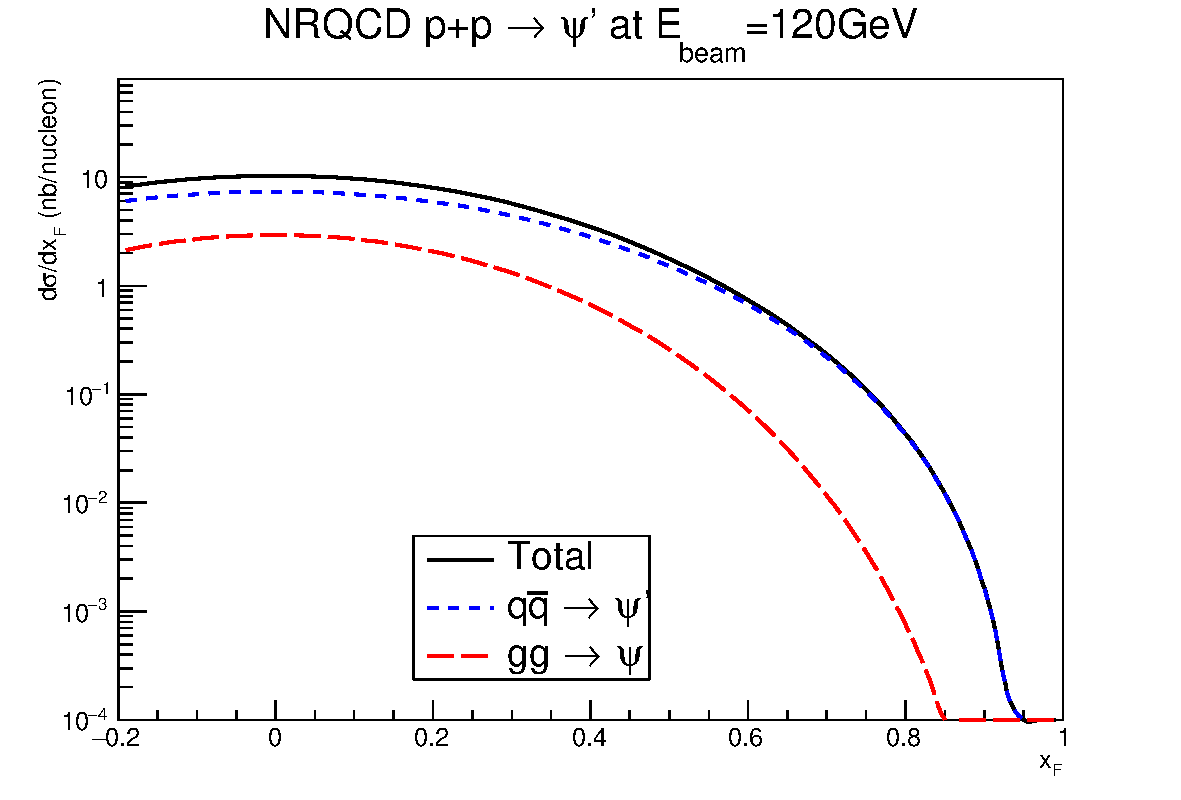
\includegraphics[width=\linewidth]{psip_cs_pp}
		\caption{$\psi'$ production.}
	\end{subfigure}
	\caption{Calculated cross section for charmonium production using NRQCD model
		\cite{chang2023a}. CT14nlo is used as the proton PDF. The LDMEs used are
		taken from Table \num{3} in Ref.~\cite{chang2023}, and are obtained from a
		global fit to fixed-target charmonium production data. }
	\label{fig:NRQCD_cs}
\end{figure}



\ifSubfilesClassLoaded{ \printbibliography[heading=bibintoc,title={References}]}{}

\end{document}
